\chapter{L'alimentazione seriale e lo ShuntLDO}
\label{AlimentazioneSeriale}
%L'alimentazione seriale dei moduli è il sistema scelto per l'alimentazione, in grado di rispettare i requisiti per il nuovo tracciatore a pixel di fase due. 
\section{Introduzione}
%Nel capitolo precedente si sono discussi i requisiti richiesti per il tracciatore di fase due: tolleranza agli alti livelli di radiazione, alta risoluzione, riduzione del materiale, etc...
%Per rispettare queste condizioni si è deciso di sviluppare un sistema di alimentazione innovativo e alternativo agli attuali convertitori DC-DC
%\footnote{
%  L'attuale tracciatore utilizza un sistema di alimentazione in parallelo dei moduli, in cui i convertitori DC-DC generano localmente le tensioni necessarie al funzionamento del chip.
%}.
%Questi, infatti, non resisterebbero ai più alti livelli di radiazione della fase ad alta luminosità, nè sarebbero in grado di operare efficacemente in presenza del campo magnetico previsto.
%Il nuovo sistema di alimentazione prevede una distribuzione seriale e sarà gestito, all'interno del chip, da circuiti dedicati prodotti in tecnologia CMOS a 65 nm.

In un sistema di alimentazione seriale~\cite{SLDO} il generatore fornisce tensione e corrente ad una catena di carichi, nel nostro caso i moduli, posti in successione. A differenza del sistema di alimentazione parallelo, in cui tutti i moduli si trovano allo stesso potenziale di riferimento e in cui la corrente totale erogata è la somma di quella che scorre nei singoli rami, nel sistema seriale la corrente totale è la stessa per tutti i moduli ed è la tensione di lavoro a cambiare. Dato che i moduli, e quindi i carichi, sono tutti nominalmente uguali, la differenza di potenziale su ciascun elemento della catena è la stessa, ma il riferimento di potenziale cambia localmente.
Inoltre, visto che la corrente viene ``riutilizzata'' in ciascun modulo, il generatore deve fornire correnti minori, rispetto a quelle di un sistema di alimentazione parallelo.
Per questo motivo le dissipazioni nei cavi sono ridotte ed è quindi possibile utilizzare cavi più sottili, riducendo il materiale presente all'interno del tracciatore.
%Questo significa che in ogni elemento scorre la medesima corrente, ma l'intervallo di tensione in cui viene a trovarsi è differente per ciascuno di essi. Fino ad ora il metodo di alimentazione utilizzato era quelo parallelo, tutti i moduli si trovano ad un potenziale comune ma su rami separati, questo implica che nel cavo principale scorre una corrente pari alla somma di quella che passa in tutti i rami e dunque sarà necessario l'utilizzo di un cavo con sezione notevolmente maggiore a quello necessario in una alimentazione seriale.
%Ciò dipende dal fatto che nel caso di alimentazione seriale la corrente sia riutilizzata n-volte riducendo così le perdite di potenza nei cavi, rispetto ad una alimentazione in parallelo, questo consente l'impiego di cavi più sottili riducendo così il materiale all'interno del tracciatore. 
%Inoltre un'alimentazione seriale, rispetto ad una in parallelo, permette di ridurre la potenza dissipata a parità del numero di moduli alimentati.

Infatti è possibile calcolare il rapporto tra la potenza assorbita da n elementi in parallelo e quella di n elementi in serie:
\begin{equation}
\mathrm{W_{parallelo} = n \cdot I \cdot V + (I\cdot n)^2 \cdot R},
\end{equation}
\begin{equation}
\mathrm{W_{serie} = n \cdot I \cdot V + I^2 \cdot R},
\end{equation}
\begin{equation}
\mathrm{\frac{W_{parallelo}}{W_{serie}} = \frac{1+ \dfrac{nRI}{V}}{1+\dfrac{RI}{Vn}}},
\end{equation}
dove R è la resistenza dei cavi, I è la corrente di alimentazione per il singolo elemento e V è la caduta di tensione su ciascun elemento. 

\section{Lo ShuntLDO per l'alimentazione seriale}
\label{sec:SLDOzener}

Nella progettazione del sistema con alimentazione seriale occorre tener conto che il consumo di ciascun ROC, anche se gli elementi della catena sono tutti identici, dipende dallo stato in cui si trova e dalle operazioni che sta eseguendo. 
Il ROC, infatti, è un carico dinamico e l'alimentazione deve essere in grado di erogare abbastanza corrente per far fronte ai picchi di assorbimento dei singoli elementi della catena.
Inoltre, le variazioni dei consumi sono molto veloci e gli alimentatori remoti, detti anche di \textit{back-end}, non sarebbero in grado di compensarle in modo rapido: questi saranno posizionati lontano dall'esperimento e i cavi, lunghi anche fino a $\sim 40-50\m$, introducono un ulteriore carico induttivo non trascurabile.

Per queste ragioni un aspetto chiave dell'implementazione di uno schema di alimentazione seriale \`e che le fluttuazioni del carico, il ROC nel nostro caso, non siano visibili esternamente ma siano gestite localmente facendo s\`i che il carico effettivo visto dalla catena sia costante. Questo pu\`o essere ottenuto implementando, in un appropriato circuito di {\em shunt}, un cammino alternativo per la corrente in quel momento non utilizzata dal ROC, tale che $\mathrm{I}_\mathrm{TOT}\sim\mathrm{I}_\mathrm{ROC}+\mathrm{I}_\mathrm{shunt}\sim\mathrm{cost}$. Inoltre \`e necessario che, in prossimit\`a del ROC, venga effettuata l'opportuna regolazione PoL, che converte l'alimentazione in corrente fornita alla catena, e quindi a ciascuno dei suoi elementi, in una alimentazione in tensione stabile, fruibile dal ROC.
\begin{figure}
\centering
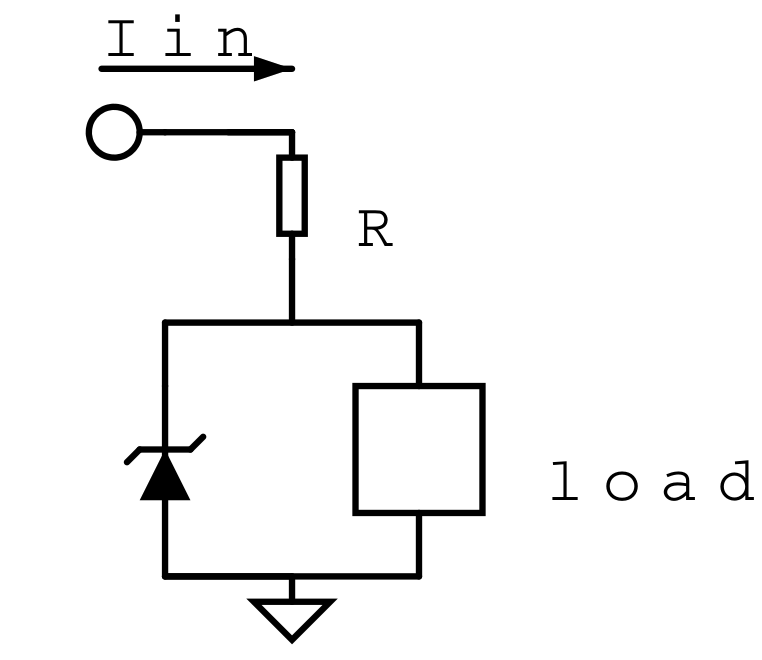
\includegraphics[width=0.5\textwidth]{Immagini/zener2}
\caption{Schema di principio di un circuito regolatore con shunt che utilizza un diodo Zener.}
\label{zener}
\end{figure}
Per flessibilit\`a, versatilit\`a e le motivazioni espresse nella Sezione~\ref{IntroROCIT} \`e auspicabile che questa elettronica addizionale sia integrata nel ROC stesso.

Un possibile schema di principio di tale circuito \`e visibile in~Fig.~\ref{zener} in cui si sfrutta un diodo Zener contropolarizzato per ottenere la stabilizzazione in tensione al carico `load'. Il funzionamento è molto semplice: la corrente in ingresso induce una caduta di tensione sulla resistenza R che, tuttavia, non impedisce di contropolarizzare il diodo Zener oltre la tensione di soglia. A questo punto sarà lo stesso diodo a mantenere la tensione ai capi del carico costante, assorbendo tutta la corrente non necessaria al carico e agendo da shunt. 
Questo schema però presenta problemi operativi nel momento in cui si mettano più regolatori in parallelo, come pu\`o essere necessario fare in applicazioni pratiche, ad esempio, nel caso di un ROC dove servono due tensioni, generalmente diverse, per la parte digitale e la parte analogica, ciascuna fornita da un regolatore diverso, oppure nel caso di un modulo dove pi\`u ROC sono alimentati in parallelo condividendo la stessa corrente in ingresso. Il diodo Zener che, per inevitabili tolleranze di fabbricazione, si trovi all'accensione ad entrare in conduzione prima degli altri assorbir\`a tutta la corrente disponibile con effetti imprevedibili e potenzialmente distruttivi. 

Per ovviare a queste criticità è stato sviluppato un regolatore \textit{Low Drop Out}\footnote{Un regolatore è definito Low Drop Out quando \`e minima la differenza tra la tensione in ingresso e quella in uscita a valle della regolazione; in particolare $\mathrm{V_{dropout}=V_{in}-V_{out}\sim 0.1-0.2 \V}$.} accoppiato ad un circuito di shunt e capace di generare localmente una tensione fissa e di adattarsi dinamicamente all'assorbimento di corrente, denominato {\em ShuntLDO}, con caratteristiche elettriche tali da superare le problematiche a cui si \`e sopra accennato.

Il regolatore ShuntLDO \`e stato inizialmente sviluppato dalla collaborazione Atlas per un suo utilizzo nell'ambito del progetto {\em Insertable B-Layer} (IBL)~\cite{IBL}. Infatti la famiglia di ROC disegnati per IBL, FE-I3~\cite{ROCFEI3} e FE-I4~\cite{ROCFEI4}, implementano entrambi circuiti ShuntLDO dimensionati per correnti totali di $\sim 0.5\A$. Pur tuttavia IBL non implementa uno schema di alimentazione seriale perch\'e ad esso fu preferito uno schema di alimentazione pi\`u tradizionale.

Il disegno dello ShuntLDO \`e stato poi tradotto in tecnologia CMOS a 65~nm dalla collaborazione RD53 per la sfida di HL-LHC: inizialmente in una versione a $\sim 0.5\A$, necessaria per valutare il dispositivo in $65\nm$, per poi arrivare alle attuali versioni dimensionate per correnti massime di $\sim 2\A$.

%Il punto chiave per una alimentazione seriale è che la corrente, che viene fatta scorrere nella catena, sia maggiore o uguale a quella necessaria per alimentare l'elemento con il consumo più alto. 
%Anche nel caso in cui tutti gli elementi della catena siano identici non è vero che avranno pari consumi, gli stessi dipendono dallo stato in cui si trova il chip e le operazioni che esegue. 
%Il chip è dunque un carico dinamico e in qualsiasi momento l'alimentazione deve essere in grado di erogare abbastanza corrente per far fronte ai picchi di assorbimento dei singoli elementi della catena. 
%Dal momento che queste variazioni sono molto veloci l'alimentatore di back-end non può essere in grado di compensarle in modo rapido\footnote{Gli alimentatori sono posizionati lontano dall'esperimentpo e dunque i cavi introducono un ritardo (proporzionale alla lunghezza degli stessi), non è quindi possibile pensare di alimentare la catena in tensione. L'alimentazione dovrà essere in corrente, a livello di chip sarà poi implementato un meccanismo di bilanciamento, che gestisca le variazioni di corrente assorbita.}. Questo è un punto critico che richiede un attento studio. 
%La soluzione al problema consiste nell'implementazione di un regolatore con shunt all'interno del chip, che generi una tensione fissa e si adatti dinamicamente all'assorbimento in corrente. 
%Per quanto detto è necessario che le fluttuazioni di carico date dal chip non siano visibili esternamente, dovranno perciò essere gestite localmente. Il circuito all'interno di ciascun chip incaricato di svolgere questo compito è il regolatore con ShuntLDO.
%\section{Alimentazione seriale con RD53A}
%Partendo dall'idea di utilizzare un'alimentazione seriale, la prima idea che si può avere, è quella di porre singoli elementi in serie, ciascuno dotati di un regolatore, questa configurazione ha però una criticità molto importante: il fallimento di un singolo elemento rende inutilizzabile l'intera catena, inquanto interrompe il flusso di corrente in tutto il ramo. 
%Va perciò implementato un metodo per ovviare a questo problema e anche per mitigare le fluttuazioni di tensione causate dai vari elementi che influiscono significativamente  sulla tensione generata localmente. Il circuito che si occupa di risolvere queste problematiche è un regolatore di tensione ShuntLDO (Shunt Low Drop Out). 
%lo schema consiste in due loop di controllo accoppiati, il primo fa si che il transistor M4 faccia passare tutta la corrente che non è consumata dal carico attivo. Mentre un voltage regulator (A1+M1) assicura che il carico attivo (nel nostro caso RD53A) sia alimentato con una tensione costante, indipendentemente dalla corrente consumata e indipendentemente dalla correte che viene immessa nella catena seriale.
% 
%\section{S$_{unt}$ L$_{ow}$ D$_{rop}$ O$_{ut}$}
%\section{ShuntLDO}


%L'altro punto di interesse nel grafico è quello definito da massima tensione e massima corrente a cui è possibile alimentare il circuito. 
%Una volta sicuri che non sarà mai utilizzata una corrente maggiore del massimo per alimentare il dispositivo, si ha la sicurezza che nemmeno la tensione massima sarà raggiunta.

\subsection{Il principio di funzionamento dello ShuntLDO}

Per descrivere il funzionamento dello ShuntLDO, partiamo da uno schema estremamente semplificato che permetta di comprendere l'idea di fondo, facendo riferimento alla Fig.~\ref{SLDOprova}. 
Come anticipato il circuito di ShuntLDO è alimentato dalla corrente $\mathrm{I_{in}}$, attraverso il nodo $\mathrm{V_{in}}$.  Della corrente in ingresso una frazione $\mathrm{I_\mathrm{ref}}$ scorrerà nel ramo di R3. Questa sarà la corrente di riferimento all'interno dello shunt, vedremo in seguito perché. 
La parte che agisce come regolatore di tensione è il mosfet M1 tramite l'amplificatore A1 che equalizza la tensione sul carico al valore di riferimento $\mathrm{V_{ref}}$ aprendo o chiudendo il gate di M1 e, dunque, facendo scorrere più o meno corrente. 
In assenza della parte di shunt ci sarebbe, quindi, un aumento di $\mathrm{I_{ref}}$ e, conseguentemente, di $\mathrm{V_{in}}$. 
%Per evitare ciò è stato implementato un ramo in parallelo al carico in cui la corrente che scorre è regolata dal mosfet M4 tramite l'amplificatore A3 che, confrontando tramite un opportuno campionamento la corrente nel ramo di M1 e 1000 volte quella nel ramo di R3, ha lo scopo di mantenere la corrente in ingresso a M1 costante. Il complesso costituito da M4 e A3 è la parte attiva dello shunt: A3 fa sì che la corrente nel ramo con M1 sia 1000 volte quella di riferimento che scorre in R3, poiché modifica $\mathrm{I_{shunt}}$ attraverso la variazione della tensione di gate del mosfet M4. 
 Per evitare ciò è implementato il complesso costituito da M4 e A3, cioè la parte attiva dello shunt: A3 fa sì che la corrente nel ramo con M1 sia 1000 volte quella di riferimento, $\mathrm{I_{ref}}$, che scorre in R3, poiché modifica $\mathrm{I_{shunt}}$ attraverso la variazione della tensione di gate del mosfet M4. 
La corrente che scorre in M1 è dunque tenuta costante anche quando si hanno variazioni dinamiche del carico.
\begin{figure}[!htbp]
\centering
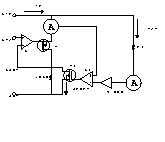
\includegraphics[width=0.75\textwidth]{Immagini/SLDObase}
\caption{Schema di principio dello ShuntLDO.}
\label{SLDOprova}
\end{figure}
 
La Fig.~\ref{SLDOprinciple} mostra graficamente il funzionamento dello ShuntLDO in cui la corrente totale circolante nella catena seriale si divide, in funzione del tempo, in quella indirizzata nello shunt e in quella richiesta dal carico, nelle sue componenti analogica e digitale; \`e esemplificata anche la situazione da evitare, ovvero la richiesta, per tempi prolungati, di una corrente maggiore rispetto a quella disponibile nella catena.
\begin{figure}[!htbp]
\centering
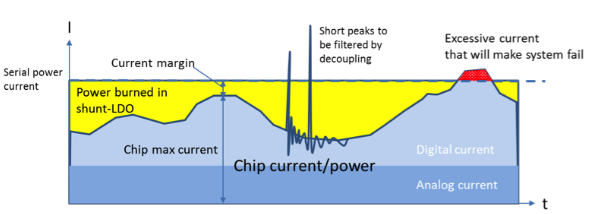
\includegraphics[width=0.75\textwidth]{Immagini/ShuntRegulatorPrinciple}
\caption{Andamento qualitativo della corrente assorbita da un ROC in funzione del tempo. Mentre la componente analogica \`e sostanzialmente costante, la componente digitale subisce variazioni, anche repentine. Sono da evitare le situazioni in cui il carico richieda, per lunghi periodi di tempo, una corrente in eccesso rispetto a quella circolante nella catena, rappresentata in giallo, mentre picchi veloci possono essere gestiti con opportuno filtraggio.}
\label{SLDOprinciple}
\end{figure}

\subsection{Lo ShuntLDO da $0.5\A$ in 65nm}

 
\begin{figure}[!htbp]
\centering
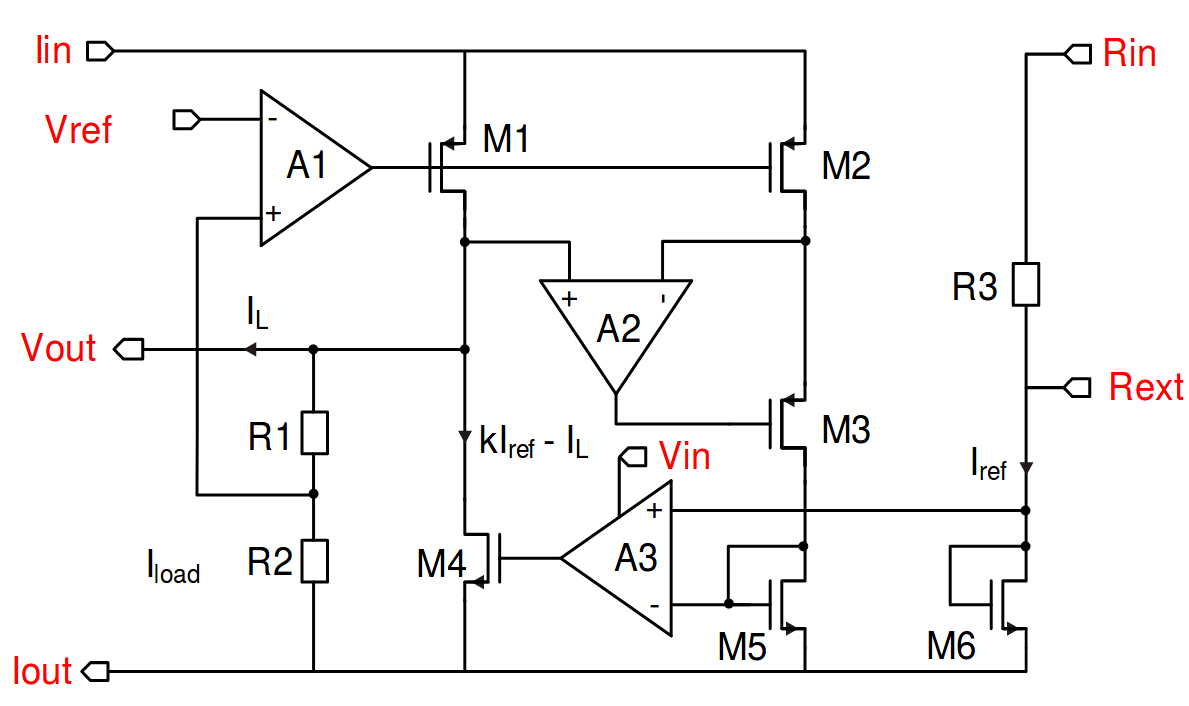
\includegraphics[width=0.95\textwidth]{Immagini/SLDO5A}
\caption{Circuito semplificato dello ShuntLDO 0.5 A.}
\label{SLDO5A}
\end{figure}

In Fig.~\ref{SLDO5A} \`e mostrato lo schema elettrico del prototipo di ShuntLDO in versione a $65\nm$ dimensionato per $0.5\A$ di corrente massima.
Rispetto a quanto visto in precedenza si hanno alcune differenze, benché l'idea generale di funzionamento rimanga la stessa. 
In questo schema il carico si trova tra i nodi $\mathrm{V_{out}}$ e $\mathrm{I_{out}}$. Grazie al partitore costituito da R1 e R2, con R1=R2, e all'amplificatore A1, $\mathrm{V_{out}}$ risulta essere il doppio della tensione di riferimento $\mathrm{V_{ref}}$.
%\footnote{$\mathrm{V_{ref}}$ non ha niente a che vedere con $\mathrm{I_{ref}}$.}
L'amplificatore A3, invece, confronta la corrente $\mathrm{I_{ref}}$ che scorre nel ramo di R3 (dato che normalmente i nodi $\mathrm{I_{in}}$ e $\mathrm{R_{in}}$ sono connessi) e quella che scorre in M2 e regola il mosfet M4 di conseguenza. 
La coppia di mosfet M1-M2 costituisce un \textit{current-mirror} configurato in modo tale che il rapporto k tra le due correnti sia uguale a 1000 grazie ad una appropriato dimensionamento dei due dispositivi\footnote{
  In un \textit{current-mirror} il rapporto k è uguale a $\dfrac{W_1L_2}{W_2L_1}$ dove $W_1$ e $L_1$ e $W_2$ e $L_2$ sono, rispettivamente, profondità e lunghezza dei due mosfet.
}. 
Grazie al \textit{current-mirror}, quindi, la corrente che scorre in M1 è 1000 volte $\mathrm{I_{ref}}$ e il sistema costituito dall'amplificatore A2 e il mosfet M3 ha lo scopo di migliorare la precisione di questo current mirror.
Questa scelta progettuale definisce il modo in cui lo ShuntLDO è visto esternamente. Infatti la corrente $\mathrm{I_{in}}$ che scorre nello ShuntLDO pu\`o essere espressa come
\begin{equation}
\mathrm{I_{in} \sim k I_{ref} \sim k \frac{V_{in} - V_{thM6}}{R_3}}
\label{eq:IV05amp}
\end{equation}
dove $\mathrm{V_{thM6}}$ \`e la tensione di soglia del mosfet M6. Quindi il generatore connesso al nodo $\mathrm{V_{in}}$ vede un carico resistivo pari a $\mathrm{\nicefrac{R3}{k}}$ in serie con una piccola tensione di offset. Il valore di R3 è, quindi, un importante parametro, la cui scelta determina la tensione nel punto di lavoro per una data corrente e, pi\`u in generale, la pendenza di $\mathrm{V_{in}}$ in funzione di $\mathrm{I_{in}}$ nella zona di regolazione, come visibile in Fig.~\ref{fig:IVSLDO} che mostra il caratteristico grafico corrente-tensione dello ShuntLDO e che approfondiremo in seguito.
Il valore di R3 \`e configurabile tramite il terminale indicato con $\mathrm{R_{ext}}$ dove è possibile collegare una resistenza esterna per alterare il valore del resistore integrato nello ShuntLDO.
\begin{figure}[!htbp]
\centering
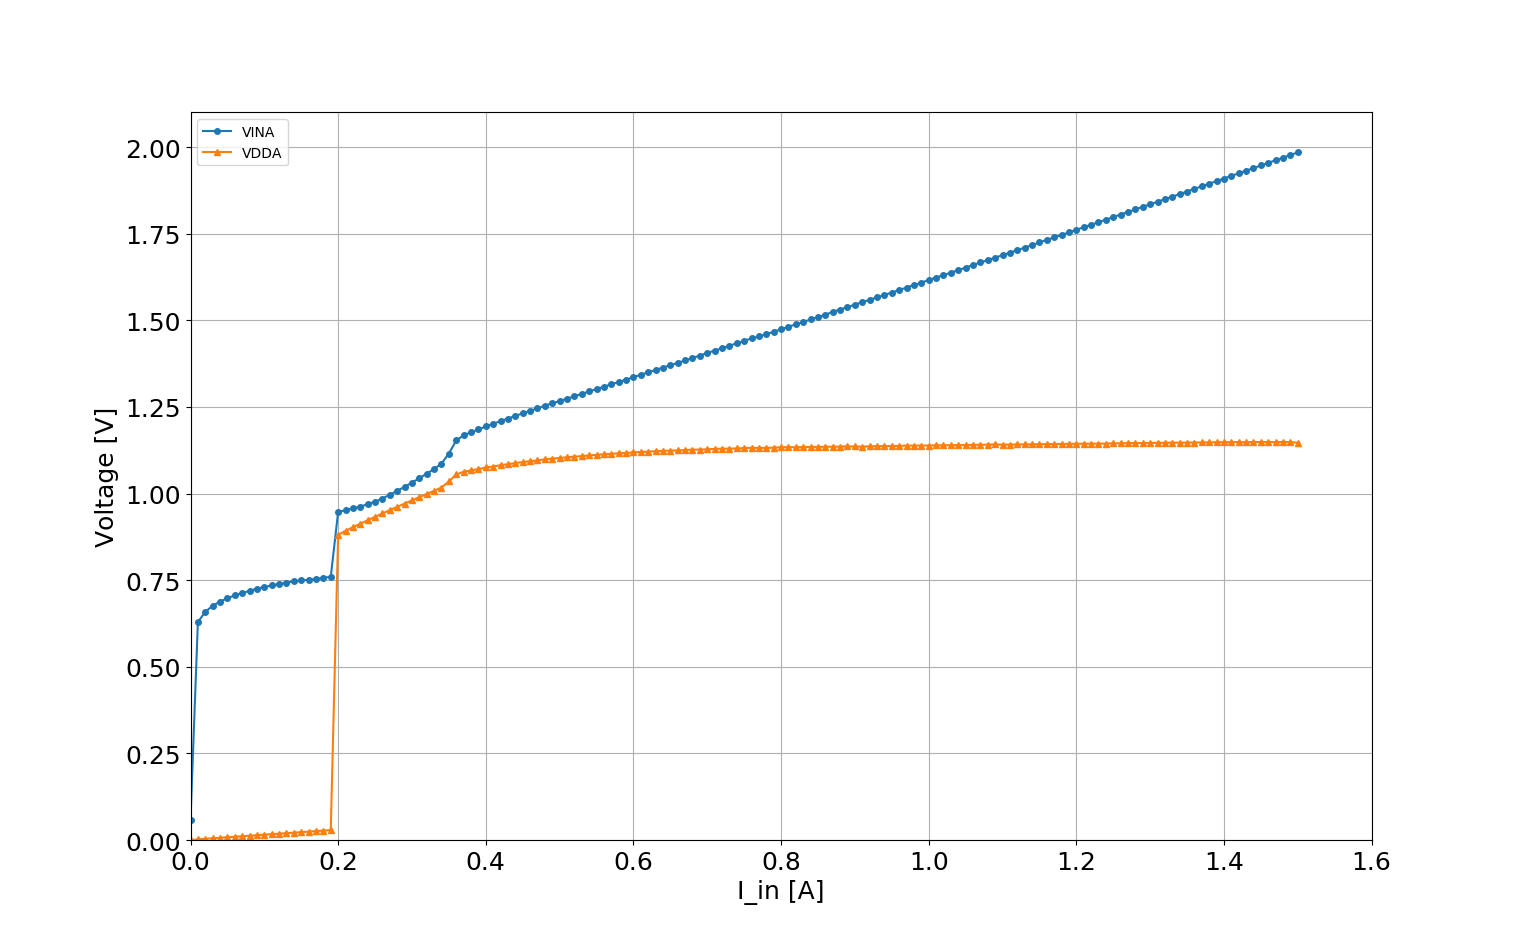
\includegraphics[width=0.99\textwidth]{Immagini/CaratteristicaSLDO.png}
\caption{Caratteristica corrente-tensione per uno ShuntLDO che mostra $\mathrm{V_{in}}$ (curva blu) e $\mathrm{V_{out}}$ (curva rossa) in funzione di $\mathrm{I_{in}}$; la regolazione di  $\mathrm{V_{out}}$ al valore di $\sim 1.15\V$ inizia per $\mathrm{I_{in}}\sim0.4\A$. Al di sopra di questo valore $\mathrm{V_{in}}$ ha una pendenza pari a $\sim\mathrm{\nicefrac{R3}{k}}$.}
\label{fig:IVSLDO}
\end{figure}

Per una corretta funzione di regolazione, lo ShuntLDO da $0.5\A$ necessita di una tensione in ingresso minima di circa $1.4-1.5\V$, a fronte di un $\mathrm{V_{out}}$ nominale pari a $\sim 1.2\V$ corrispondente, entro qualche decina di mV, al valore di tensione necessario sia per la componente analogica che per la componente digitale del futuro ROC per l'IT. Il rapporto della differenza tra tensione di ingresso e tensione di regolazione, pari a $\sim 200\mV$, con la tensione in ingresso rappresenta una stima della potenza minima dissipata dallo ShuntLDO pari, quindi, al $\sim 15-20\%$. A parit\`a di $\mathrm{I_{in}}$ e di $\mathrm{V_{out}}$, la scelta della resistenza R3 definisce $\mathrm{V_{in}}$ e, quindi, il punto di lavoro dello ShuntLDO in termini della potenza in eccesso che \`e necessario fornire al regolatore.
\FloatBarrier

% Valori di resistenza maggiori consentiranno, quindi, di operare con correnti minori, con il vantaggio di consumare minor potenza\footnote{
%   La corrente in ingresso è fissata e quella non utilizzata viene dissipata sullo shunt, che diventa conseguentemente molto caldo.
% },
% ma con lo svantaggio di aver minor spazio per le fluttuazioni del carico. 
% Analogamente resistenze minori avranno l'effetto contrario: tensioni minori con correnti maggiori.

\subsection{Lo ShuntLDO da $2\A$ in 65nm}
\label{ShuntLDO2A}

La successiva versione del prototipo di ShuntLDO a 65nm, progettata per correnti nominali di $2\A$, implementa un ulteriore parametro di configurazione della caratteristica IV per una maggiore flessibilit\`a di utilizzo e configurazione. In particolare \`e stata aggiunta una parte circuitale che permette di calibrare la tensione di offset che definisce la corrente di riferimento nella resistenza R3, pari semplicemente a $\mathrm{V_{thM6}}$, nella versione precedente. Nella Fig.~\ref{SLDO2A}, che mostra lo schema elettrico dello ShuntLDO da $2\A$, \`e visibile il complesso aggiunto per questo scopo costituito dal mosfet M7 controllato dall'amplificatore A4.
\begin{figure}[!htbp]
\centering
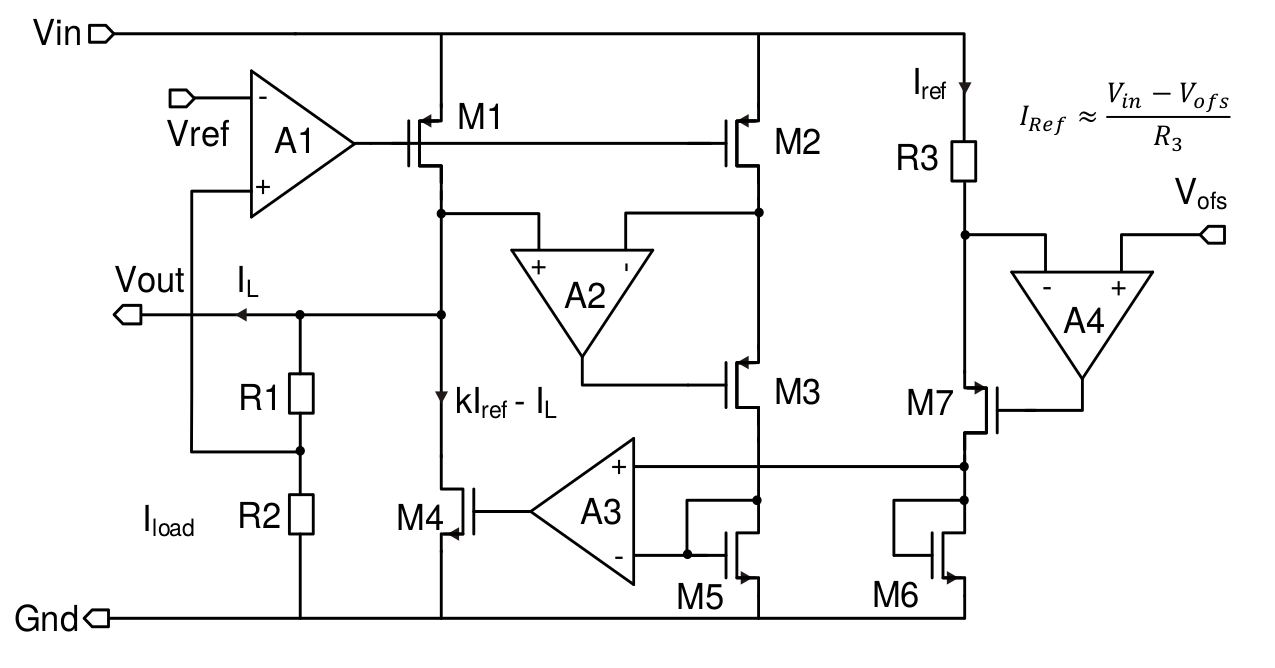
\includegraphics[width=\linewidth]{Immagini/SLDO2A}
\caption{Circuito semplificato dello ShuntLDO 2A.}
\label{SLDO2A}
\end{figure}
%Per quanto visto fin ora non c'è traccia della possibilità di avere un offset.
%In questo tipo di schematico non è prevista la possibilità di avere una $\mathrm{V_{offset}}$.
%Questa caratteristica è stata introdotta nel prototipo a $2A$ riportato in figura \ref{SLDO2A}.
%Facendo riferimento a questa, si può vedere che, rispetto alla versione a $0.5A$, è presente il mosfet M7 sul ramo di R3, il cui gate è controllato da A4.
Grazie alla presenza di questo ulteriore stadio, la corrente di riferimento $\mathrm{I_{ref}}$ diventa, quindi,
\begin{equation}
\mathrm{I_{ref} = \frac{V_{in} - V_{ofs}}{R_3}},
\end{equation}
dove $\mathrm{V_{ofs}}$ \`e la tensione di offset definita tramite l'omonimo terminale, da cui segue una relazione tra $\mathrm{V_{in}}$ e $\mathrm{I_{in}}$ leggermente modificata rispetto alla Eq.~\ref{eq:IV05amp}: 
\begin{equation}
\mathrm{I_{in} \sim k I_{ref} \sim k \frac{V_{in} - V_{ofs}}{R_3}}.
\end{equation}
La tipologia circuitale dello ShuntLDO a $2\A$ \`e, per il resto, invariata rispetto all'omologo a $0.5\A$. La pi\`u ampia tolleranza in corrente \`e ottenuta grazie al dimensionamento dei mosfet M1 e M4 e ad altri dettagli di implementazione del circuito in tecnologia CMOS.

\subsection{Lo ShuntLDO: il circuito equivalente}

Da quanto descritto nelle sezioni precedenti si pu\`o definire regione operativa, o di regolazione dello ShuntLDO, quell'ambito in cui la corrente $\mathrm{I_{in}}$ \`e tale per cui $\mathrm{V_{in}\gtrsim 2\times V_{ref}}+{\cal O}\mathrm{(200\mV)}$, e quindi $\mathrm{V_{out}\sim 2\times V_{ref}}$, e, al contempo, $\mathrm{V_{in}\lesssim V_{in}^{MAX}}$, dove $\mathrm{V_{in}^{MAX}\sim2.0\V}$ è il valore limite per un circuito basato su tecnologia CMOS a $65\nm$. In questa regione il comportamento dello ShuntLDO rispetto ai terminali di ingresso \`e schematizzabile come una resistenza efficace, $\mathrm{R_{eff}}$, definita da $\mathrm{\nicefrac{R3}{k}}$, in serie ad un generatore di tensione, $\mathrm{V_{offset}}$. Le variazioni di corrente utilizzata dal reale carico attivo, il ROC nel nostro caso, non sono quindi visibili esternamente al regolatore.
%Un importante caratteristica di questo particolare circuito è che esternamente è visto come una resistenza efficace $\mathrm{R_{eff}}$, in serie ad un offset di tensione $\mathrm{V_{offset}}$, mentre il carico attivo, nel nostro caso il chip RD53A, non è visibile e dunque non lo sono nemmeno le sue le sue variazioni. 
Il comportamento resistivo permette l'utilizzo di più ShuntLDO in parallelo fra di loro, con la corrente che si suddivide in base alla resistenza efficace di ciascuno. La resistenza equivalente risultante \`e quella del parallelo delle resistenze efficaci dei singoli dispositivi superando cos\`i le problematiche descritte nella Sezione~\ref{sec:SLDOzener} che affliggono un tradizionale circuito shunt basato su diodo Zener.

%Inoltre, utilizzando resistenze esterne, è possibile scegliere il valore di $\mathrm{R_{eff}}$ e, conseguentemente, la quantità di corrente che scorre in ciascun elemento posto in %parallelo.

Lo ShuntLDO pu\`o essere implementato direttamente sul ROC stesso e questo ne rappresenta uno degli innegabili vantaggi sia in termini di miniaturizzazione, sia in termini di prossimit\`a al carico reale della regolazione PoL. Come menzionato, gi\`a i ROC per Atlas IBL (FE-I3 e FE-I4) ospitavano due ShuntLDO~\cite{SerialPowering}, uno per la tensione analogica e uno per la tensione digitale. La collaborazione RD53 ha recentemente realizzato il ROC RD53A\cite{RD53A}, il primo prototipo del ROC per HL-LHC, destinato ad essere utilizzato per ampi studi di R\&D. Anche RD53A, che sar\`a descritto nel capitolo~\ref{cap:RD53A}, implementa due ShuntLDO destinati all'alimentazione analogica e all'alimentazione digitale. In condizioni normali questi ShuntLDO lavoreranno in parallelo condividendo la corrente in ingresso. La scelta dei rispettivi valori di $\mathrm{R_{eff}}$ definisce la suddivisione di corrente nei due domini. A differenza dei ROC della passata generazione, in cui il consumo di corrente della parte digitale era marginale rispetto alla parte analogica, in RD53A la componente analogica e quella digitale avranno consumi confrontabili. Per questo motivo i due ShuntLDO sono configurati in modo analogo.

La Fig.~\ref{VVC} mostra l'andamento della tensione $\mathrm{V_{in}}$ in funzione della corrente totale $\mathrm{I_{in}}$ fornita al ROC assumendo la caratteristica ideale corrente-tensione sopra descritta. Sono, inoltre, evidenziati i valori operativi massimi e la tensione minima di lavoro.
\begin{figure}[!htbp]
\centering
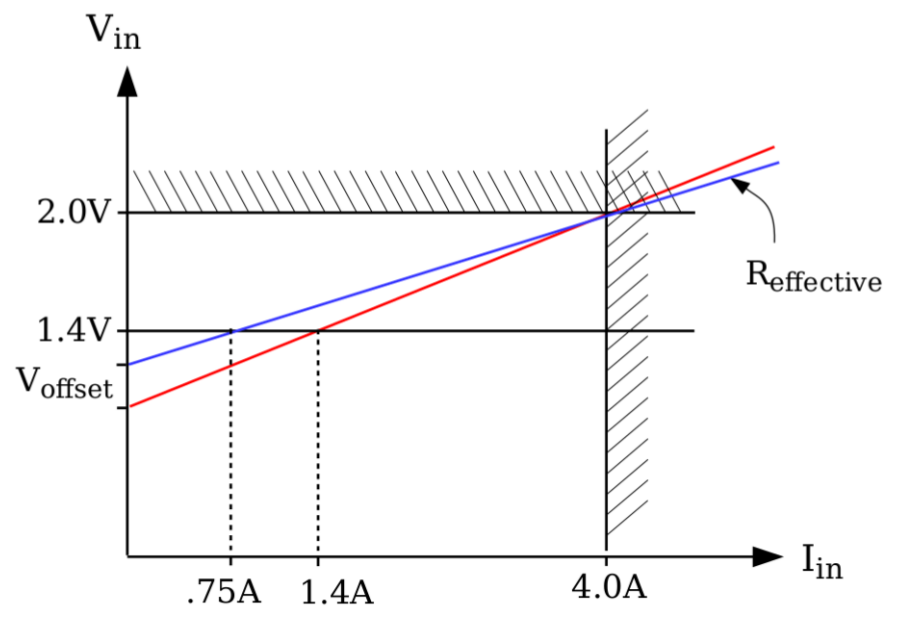
\includegraphics[width=0.75\textwidth]{Immagini/VoltageVsCurrent}
\caption{Andamento della tensione in funzione della corrente per il ROC. Le zone tratteggiate sono oltre i valori operativi massimi (4.0 A per la corrente e 2.0 V per la tensione), la linea orizzontale a 1.4 V è la tensione minima di lavoro, la pendenza è la resistenza efficace. Combinazioni differenti di resistenza e offset consentono di spostare il punto di lavoro.}
\label{VVC}
\end{figure}
In particolare vengono illustrati i criteri di scelta per i valori di $\mathrm{R_{eff}}$ e $\mathrm{V_{offset}}$: da un lato \`e necessario avere una corrispondenza fra la massima corrente erogabile ($4.0\A$ per il parallelo dato che il singolo ShuntLDO tollera una corrente massima di $\sim2\A$) e la massima tensione ($2.0\V$), dall'altra si dovrà far s\`i che la corrente corrispondente alla tensione minima di lavoro ($1.4\V$) sia sufficiente per il funzionamento del ROC tenendo anche conto di un certo margine necessario per sopperire a eventuali fluttuazioni nei consumi. Sempre in Fig.~\ref{VVC}  sono visibili due possibili combinazioni $\mathrm{R_{eff}}$ e $\mathrm{V_{offset}}$ rappresentate come due diverse caratteristiche IV.

% Una volta scelti i valori di $\mathrm{R_{eff}}$ e $\mathrm{V_{offset}}$, il consumo in potenza è completamente definito da:
% %La scelta di $\mathrm{R_{eff}}$ e $\mathrm{V_{offset}}$ definisce il consumo in potenza:
% \begin{equation}
% \mathrm{W=I_{in}^2R_{eff}+I_{in}V_{offset}}
% \end{equation}
% %una $R_{eff}$ minore consente di avere minor aumento di potenza all'aumentare della corrente. 
% %e dunque per un corretto funzionamento del chip è possibile utilizzare correnti minori, ovvero lasciando meno margine per le fluttuazioni, proprio perchè con $r_{eff}$ minore le fluttuazioni di corrente
% Accenniamo qui al fatto che la possibilità di modificare $\mathrm{R_{eff}}$ e $\mathrm{V_{offset}}$ permette di progettare diverse configurazioni di consumo in relazione alle necessità.
% Ad esempio si potrebbe avere un \textit{high power mode}, in cui la corrente alla tensione minima di lavoro sia sufficiente a garantire il funzionamento dei chip accesi e funzionanti alle massime prestazioni, come potrebbe essere il caso della linea rossa in figura \ref{VVC}, e un \textit{low power mode} in cui la stessa sia minore poiché non si richiede il funzionamento ``completo'' dei chip, come ad esempio rappresentato dalla linea blu in Figura \ref{VVC}.


% %Con questo tipo di configurazione la corrente erogata dagli alimentatori di back-end deve essere maggiore o uguale a quella necessaria all'elemento con consumo più alto.

% %La posibilità di modificare $\mathrm{R_{eff}}$ e $\mathrm{V_{offset}}$ apre alla possibilità di progettare un modo per avere diverse configurazioni, una di low-power mode e una high power mode. %Al fine di ridurre il consumo di potenza, la resistenza effettiva dello SLDO può avere un offset modificabile. 
% %(Low-power mode configuration, che cosa posso dire...).




\subsection{Schema di catena di alimentazione con ShuntLDO}

\begin{figure}
\centering
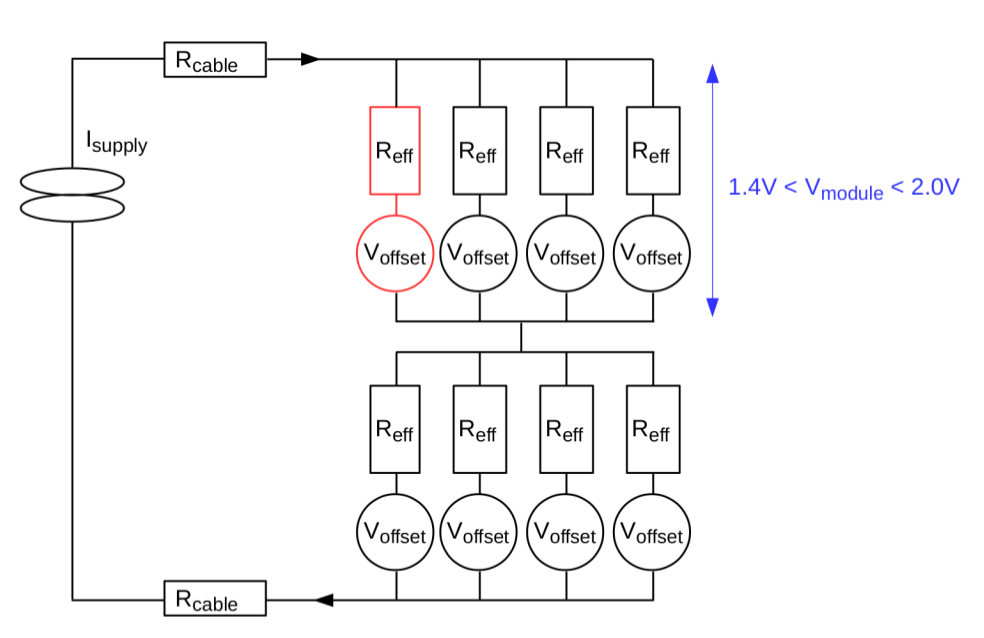
\includegraphics[width=0.75\textwidth]{Immagini/MultiChipModules}
\caption{Schema di una catena seriale con due moduli da quattro ROC. Il ramo con $\mathrm{R_{eff}}$ e $\mathrm{V_{offset}}$ in colore rosso rappresentano un ROC malfunzionante, non pi\`u attraversato da corrente, come discusso nel testo.}
\label{MCM}
\end{figure}

Il disegno dell'IT prevede moduli \modud\ e \moddd\ organizzati in catene di alimentazione seriale composte da 8-12 moduli. I due o quattro ROC di ciascun modulo sono alimentati in parallelo. Lo schema equivalente di due moduli da quattro ROC posti in serie \`e mostrato in Fig.~\ref{MCM} dove $\mathrm{R_{eff}}$ e $\mathrm{V_{offset}}$ rappresentano, a loro volta, il circuito equivalente al parallelo dei due ShuntLDO che sovrintendono, rispettivamente, alla alimentazione analogica e alla alimentazione digitale.

Nella fase progettuale era stata valutata anche la possibilit\`a di implementare l'alimentazione seriale concatenando in serie 8-12 ROC singoli; la catena sarebbe cio\`e costituita da un certo numero di moduli in serie con i ROC di ciascun modulo concatenati in serie anch'essi. Un tale approccio \`e stato scartato perch\'e il sensore si troverebbe ad operare con i pixel polarizzati ad una tensione differente a seconda del ROC a cui sono connessi con effetti che non sono stati valutati a fondo e che, molto probabilmente, richiederebbero uno specifico disegno delle strutture del sensore.

Studiamo adesso l'andamento dei consumi dovuti a più moduli in serie e come cambiano nel caso di un malfunzionamento di uno di questi (per esempio al livello del regolatore) in seguito al quale si azzera la corrente che scorre nel relativo ramo.
%Per meglio comprendere i risvolti dati dall'utilizzo di un'alimentazione seriale con SLDO è interessante fare un esempio dei consumi di questo tipo di alimentazione. 
A titolo di esempio, quindi, prendiamo la situazione in cui si ha una catena seriale costituita da 8 moduli da 4 ROC ciascuno; 
% questo per far si che nel caso un regolatore si guasti , la corrente possa essere assorbita da un altro regolatore all'interno del modulo\footnote{Come già detto i regolatori devono essere in grado d lavorare in parallelo, generare differenti tensioni dalle correnti in ingresso e tenere costante il consumo di corrente tramite lo shunt.}. 
assumiamo che il punto di lavoro scelto corrisponda a $\mathrm{R_{eff}=0.3\Ohm}$ $\mathrm{V_{offset}=0.8}\V$ per il parallelo tra lo ShuntLDO `analogico' e lo ShuntLDO `digitale' dato che la resistenza equivalente di un singolo ShuntLDO \`e tipicamente $0.6\Ohm$.
%Prendiamo come modello la situazione in cui si ha un serie di 8 moduli con 4 chip ciascuno, assumiamo che $\mathrm{V_{offset}=0.8} \V$ e $\mathrm{R_{eff}=0.3}$ $\Omega$ per ciascun chip\footnote{$\mathrm{R_{eff}}$ del singolo SLDO è circa 0.600 $\Omega$, nel chip sono presenti due SLDO in parallelo uno per l'alimentazione della parte digitale ed uno per quella analogica. La $\mathrm{R_{eff}}$ con cui viene visto il chip è dunque la metà, 0.300 $\Omega$.}. 
Con una corrente di lavoro totale richiesta di $\mathrm{I^{ROC}_{in}\sim2.0}\A$ per ROC, equamente divisa tra parte analogica e parte digitale, la corrente totale da fornire all'intero modulo \`e $\mathrm{I_{in}^{modulo}\sim8.0}\A$ corrispondente a $\mathrm{V_{modulo}=1.4} \V$.

Rispetto a questo valore nominale la corrente circolante nella catena deve essere incrementata per avere un opportuno margine di gestione dei picchi di carico da parte del ROC a valle del regolatore. Come si vedr\`a pi\`u avanti, per esempio in Fig.~\ref{LoadTransient}, per avere stabilit\`a della regolazione \`e ragionevole avere un $\sim20-25\%$ di corrente in pi\`u rispetto al valore nominale.
% Per avere un po' di margine incrementiamo la corrente di un 20$\%$, la scelta di dare un margine del 20$\%$, piuttosto che del 40$\%$ è una scelta giustificata qualitativamente dall'ampiezza dei picchi di tensione generati dallo SLDO in concomitanza di un transiente, in figura \ref{LoadTransient} è riportato il valore di picco dell'undershoot/overshoot in funzione del margine di corrente dato su 1 A di alimentazione.
% \begin{figure}
% \centering
% 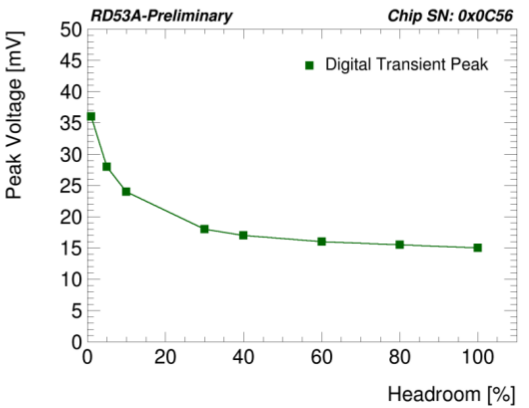
\includegraphics[width=0.75\textwidth]{Immagini/LoadTransientDominik}
% \caption{Il grafico riporta il valore di picco dell'undershoot/overshoot in funzione del margine di corrente dato su 1 A di alimentazione nel caso in cui  i consumi di parte analogica e digitale sono entrambi $\sim$0.5 A, 100$\%$ significa che la corrente fornita al chip è 1 A+1 A.}
% \label{fig:LoadTransient}
% \end{figure}
Conseguentemente $\mathrm{I^{ROC}_{in}=2.4}\A$, $\mathrm{I_{in}^{modulo}=9.6}$ A, $\mathrm{V_{modulo}\sim1.5} \V$ (per un consumo totale di $\sim14.4\W$ per modulo) e, quindi, la caduta di tensione su tutta la catena, formata da 8 moduli, sarà $\sim 12\V$.
%Con una corrente di $\mathrm{I_{in}=2.0}$ A per chip\footnote{Che vale a dire 1 A per ciascuno dei due SLDO presenti nel chip.} ($\mathrm{I=8.0}$ A per modulo) si avrà un $\mathrm{V_{modulo}=1.4} \V$, per avere un po' di margine incrementiamo la corrente di un 20$\%$, la corrente che arriva nei moduli sarà I = 9.6 A. 
%In questa situazione $\mathrm{V_{modulo}=1.52}$ V e dunque la caduta di tensione su tutta la catena formata da 8 moduli sarà pari a $12.16 \V$. Questa non è la caduta di tensione totale, va tenuto conto anche della resistenza dovuta ai cavi, in questo esempio assumiamo valga 2 $\Omega$. 
%Tenendo conto anche della resistenza dovuta ai cavi, che assumiamo valga $2 \Ohm$,
La tensione fornita dal generatore remoto sar\`a $\sim 14-15\V$ perch\`e si dovr\`a tener conto anche della dissipazione sui cavi che si stima compresa tra il $15$ e il $20\%$, comunque ben inferiore ai valori tipici di uno schema di alimentazione parallelo.
%Il generatore sarà infine $\mathrm{V \sim I_{in}^{modulo} \cdot 2 \Ohm +12 \V \sim 31 \V}$.
 
% Dai conti fatti risulta che circa il $60 \%$ della potenza è dissipata sui cavi\footnote{
%  Nonostante il valore elevato in assoluto, bisogna tenere presente che è in realtà un miglioramento rispetto alla situazione attuale, nella quale l'alimentazione è in parallelo.
%}. % sarebbe carino sapere la percentuale di consumo attuale
%La tensione di uscita del generatore è dunque $\mathrm{V=I \cdot 2 \Omega +12.6 \V=31.8 \V}$\footnote{Circa il $60 \%$ della potenza è dissipata sui cavi, questo fatto potrebbe sembrare un pessimo traguardo, in realtà è un miglioramento rispetto alla situazione attuale, nella quale l'alimentazione è in parallelo.}.% sarebbe carino sapere la percentuale di consumo attuale

% Il generatore posto a monte della catena è limitato in corrente e, per fare sì che la potenza erogabile sia maggiore di quella necessaria alla catena, si pone il valore limite della tensione leggermente superiore a quello fin qui calcolato, diciamo ad esempio 34 V.
% %In questo sistema il generatore a monte della catena sarà limitato in corrente, mentre il limite per la tensione sarà posto leggermente maggiore a quello minimo, ad esempio 34 V. 
% %In questo modo la potenza che il generatore può erogare è maggiore di quella necessaria per la catena. 
% La potenza massima che il generatore potrà erogare è, quindi, di $34 \V \cdot 9.6$ A = 326.4 W, per cui, sottraendo la potenza dissipata sui cavi e dividendo per il numero di moduli, si ottiene una potenza per modulo di 17.76 W
% \footnote{
%   Questo a fronte di una potenza assorbita, nelle normali condizioni di lavoro, di
%   \begin{equation*}
%     \mathrm{W_{modulo} = 4 \cdot W_{chip} = I_{modulo} \cdot V_{modulo} = 14.6 W}
%   \end{equation*}
%   per modulo.
% }.
% %Vedremo infatti, come questo sia necessario utile nel caso in cui alcuni chip smettano di funzionare. 
% %La potenza massima erogabile dal generatore sarà $34 \V \cdot 9.6$ $A = 326.4$ W, sottraendo la potenza dissipata sui cavi e dividendo per il numero di moduli si ottiene una potenza per modulo di $17.76$ W. Questo a fronte  di una potenza assorbita, nelle normali condizioni di lavoro, di $\mathrm{W = 4 \cdot W_{chip} = I \cdot V_{modulo} = 14.6}$ W per modulo.

Una accurata valutazione dei malfunzionamenti della catena seriale non \`e ancora stata fatta nell'ambito del progetto IT. Questa infatti non pu\`o prescindere dalla realizzazione di catene prototipali estese, attivit\`a prevista nei prossimi mesi. Ipotizziamo tuttavia che, a seguito di un danneggiamento, gli ShuntLDO di un ROC non siano pi\`u attraversati da corrente come mostrato in Fig.~\ref{MCM} dal ramo con $\mathrm{R_{eff}}$ e $\mathrm{V_{offset}}$ rappresentati in colore rosso.
% Vediamo a questo punto cosa accade nel caso in cui uno dei chip in uno dei moduli sia fuori uso
% \footnote{
%   Dal momento che nel chip ci sono due SLDO, in realtà lo scenario più probabile è che solo uno dei due sia danneggiato.
% },
%Vediamo a questo punto cosa accade nel caso in cui un chip in uno dei moduli sia fuori uso\footnote{Dal momento che nel chip ci sono due SLDO, in realtà lo scenario più probabile è che solo uno dei due sia danneggiato.}.
Ciascuno dei tre ROC dello stesso modulo rimanenti dovrà quindi farsi carico della corrente che non attraversa pi\`u il modulo danneggiato per una corrente totale per ROC pari a $\mathrm{I_{in}^{modulo}/3 \sim 3.2 A}$, valore corrispondente a un terzo di corrente in più rispetto ai $2.4\A$ nominali.
%Dato che l'alimentazione è in corrente, ciascuno dei tre chip rimanenti dovrà assorbire un terzo di corrente in più, dunque la corrente per ciascun chip sarà $\mathrm{I = 9.6A / 3 = 3.2 A}$. 
Di conseguenza cambier\`a anche la caduta di tensione sul modulo in questione che sarà 
\begin{equation*}
  \mathrm{V_{modulo} = 3.2\A \cdot 0.3 \Omega + 0.8\V = 1.8 \V},
\end{equation*}
e la potenza dissipata
\begin{equation*}
  \mathrm{W_{modulo} = 3 \cdot W_{chip} = 3 \cdot I \cdot V_{modulo} = I_{modulo} \cdot V_{modulo} = 16.9W},
\end{equation*}
con un incremento di $\sim2.5\W$ per il singolo modulo, corrispondente a circa il $17\%$. Sul totale della catena, questa maggior richiesta di potenza \`e dell'ordine del \% e quindi marginale. Un ulteriore malfunzionamento porterebbe la caduta di tensione sul modulo a $\mathrm{V_{modulo} = 4.8\A \cdot 0.3 \Omega + 0.8\V = 2.2 \V}$, quindi oltre la soglia di tolleranza in tensione della tecnologia CMOS a $65\nm$ con la conseguenza di avere l'imminente rottura anche degli ulteriori due ROC. La situazione \`e in generale assai pi\`u critica per i moduli \modud\ dato che, in caso di malfunzionamenti, il ROC rimanente si troverebbe a gestire il doppio della corrente nominale.

Si spera per\`o che risulti chiaro da questi esempi che la scelta del punto di lavoro (e quindi di  $\mathrm{R_{eff}}$ e $\mathrm{V_{offset}}$) \`e di importanza fondamentale non solo per le condizioni operative standard, ma anche per la gestione dei malfunzionamenti che spostano localmente il punto di lavoro dei regolatori adiacenti. Non \`e detto per\`o che il meccanismo di rottura pi\`u frequente sia quello in cui il ROC e i suoi regolatori non sono pi\`u attraversati da corrente; \`e ipotizzabile che gli scenari pi\`u frequenti di rottura coinvolgano il solo ROC vero e proprio e che quindi gli ShuntLDO ad esso relativi continuino a funzionare. In questo caso l'inconveniente \`e che tutta la potenza viene dissipata sui mosfet M4 dei regolatori. Per questo motivo nell'implementazione reale dello ShuntLDO sul ROC RD53A e versioni successive, la parte di potenza (essenzialmente il ramo costituito da M1 e M4) \`e ottenuta da un certo numero di repliche connesse in parallelo e distribuite sulla superficie del ROC per evitare un potenziale `hot spot' sia in condizioni standard di funzionamento che in caso di malfunzionamenti.

% Per la catena di 8 moduli l'incremento è, invece, di appena $1.7\%$.
% %Questo porta ad una caduta di tensione sul modulo $\mathrm{V_{modulo} = 3.2 A \cdot 0.3 \Omega + 0.8 V = 1.76 \V}$ e una potenza dissipata $\mathrm{W = 3 \cdot W_{chip} = 3 \cdot I \cdot V_{modulo} = 16.9}$ W, con un incremento di 2 W per il singolo modulo, che corrisponde al $13 \%$. Per la catena di 8 moduli l'incremento, invece, è di appena $1.7\%$. 
% Inoltre ci sarà anche un lieve aumento della tensione erogata dal generatore, $\mathrm{V=I \cdot 2 \Omega +14.08 \V=33.28 \V}$, che è comunque al di sotto dei 34 V
% \footnote{
%   Come visto alla tensione massima di  34 V il generatore riesce a distribuire una potenza di $17.76$ W per ciascun modulo.
% }
% impostati.
%Questo causerà anche un lieve aumento della tensione erogata dal generatore, che però rimarrà al di sotto dei 34 V\footnote{Come visto alla tensione massima di  34 V il generatore riesce a distribuire una potenza di $17.76$ W per ciascun modulo.}.
 %mettere un recap con il senso di questi conti
%Lo studio dell'alimentazione seriale parte dunque dalla caratterizzazione dello SLDO. Componente che sarà poi utilizzato all'interno del chip RD53A per la generazione delle tensioni di alimentazione della parte analogica e digitale. .......continuare discorso....
%Aver chiaro come il chip viene visto esternamente e quali siano i suoi consumi è importante per poter progettare al meglio il sistema di alimentazione seriale.
%capitolo
%\section{Prova}



%At module level, the current to voltage conversion should
%be done using more than one regulator, and by connecting all regulators in parallel. In this
%way, should one regulator fail, the current flow can still be assured by the other regulators on
%module. Although these measures assure a very robust design, extra care has to be taken for
%possible worst case failures, in particular for the case of regulator faults which could cause an
%over-voltage

%\subsection{PCB}
%
%Fino ad ora ci siamo limitati alla descrizione del funzionamento dello SLDO.
%Prima di procedere alla presentazione di misure introduciamo brevemente la (\textit{Printed Circuit Board}) di test, nella cui parte centrale è stato collocato e connesso, con wire-bond, lo ShuntLDO.
%La PCB riportata in figura \ref{PCBTestSLDO} è quella relativa al prototipo di ShuntLDO da 2A.
%La PCB è fornita di tutto ciò che è necessario al funzionamento dello SLDO e all'esecuzione dei test basilari: sono presenti connettori molex per l'alimentazione, jumper di configurazione, pin per misurare varie tensioni, etc....
%\begin{figure}
%\centering
%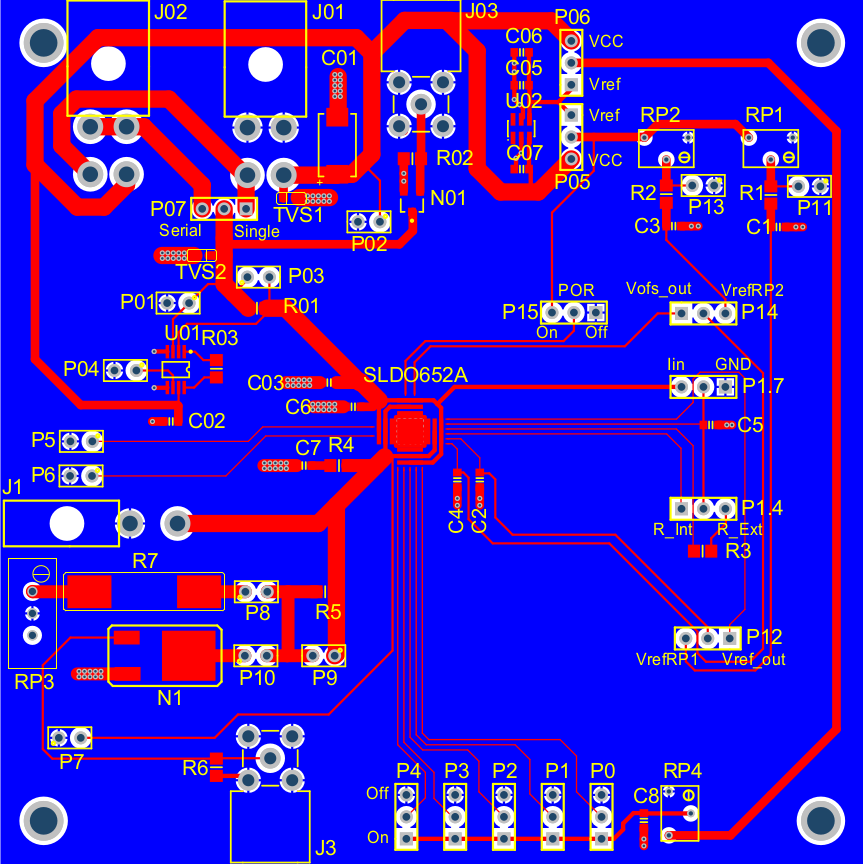
\includegraphics[scale=.3]{Immagini/chipcard}
%\caption{PCB di Test per lo SLDO 2A.}
%\label{PCBTestSLDO}
%\end{figure}

\chapter{La caratterizzazione dello ShuntLDO}

In questo capitolo viene illustrata e discussa la corposa attivit\`a effettuata nell'ambito di questo lavoro di tesi per la caratterizzazione dell'elemento circuitale ShuntLDO introdotto nel capitolo precedente. Questa attivit\`a \`e di cruciale importanza per acquisire confidenza con l'innovativo approccio dell'alimentazione seriale e con la componentistica che la rende possibile e per verificare che il comportamento in contesti realistici sia compatibile con gli stringenti requisiti imposti dalle condizioni operative di HL-LHC. Questo lavoro sar\`a ulteriormente ampliato nei prossimi mesi includendo i fondamentali test di irraggiamento, qui non contemplati, e le pi\`u ampie prove di sistema su allestimenti prototipali pi\`u estesi.

\section{Lo ShuntLDO da $0.5\A$}

Riportiamo in questo paragrafo alcune misure effettuate sul prototipo di ShuntLDO da $0.5\A$ che hanno permesso di prendere confidenza con i concetti dell'alimentazione seriale e con l'utilizzo dello ShuntLDO.
%A differenza della versione a $2\A$, in questa non è possibile inserire un valore di offset regolabile al $\mathrm{V_{out}}$.

Questo prototipo nasce come un singolo ASIC realizzato per la verifica e la validazione del solo ShuntLDO. Per il test il chip viene montato e microsaldato su una scheda di test progettata appositamente e molto versatile. In Fig.~\ref{PCB05A} sono visibili la struttura e una foto del chip stesso, che contiene tre repliche del circuito ShuntLDO, e il disegno del circuito stampato della scheda di test.
\begin{figure}
\centering
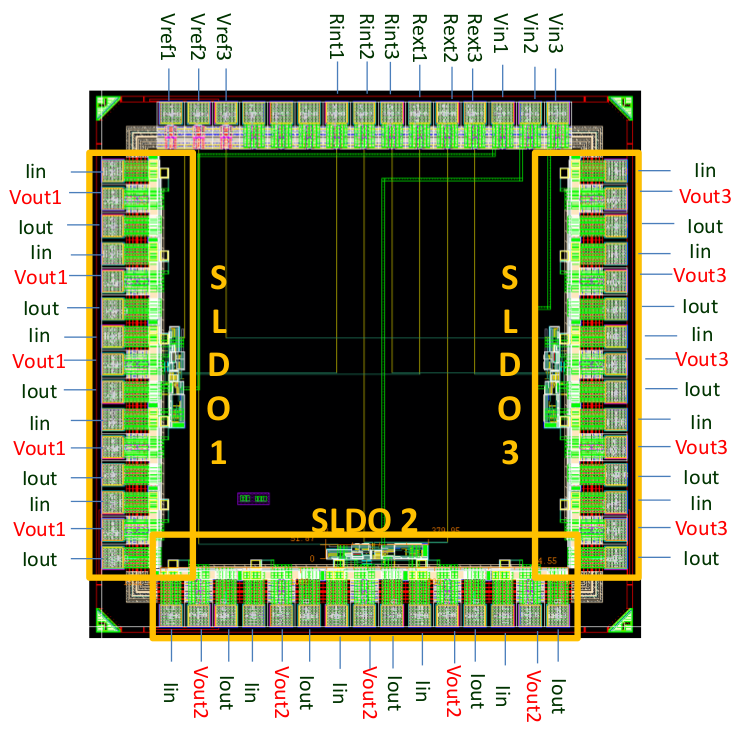
\includegraphics[width=0.32\textwidth]{Immagini/chipSLDO05A.png}
\hfill
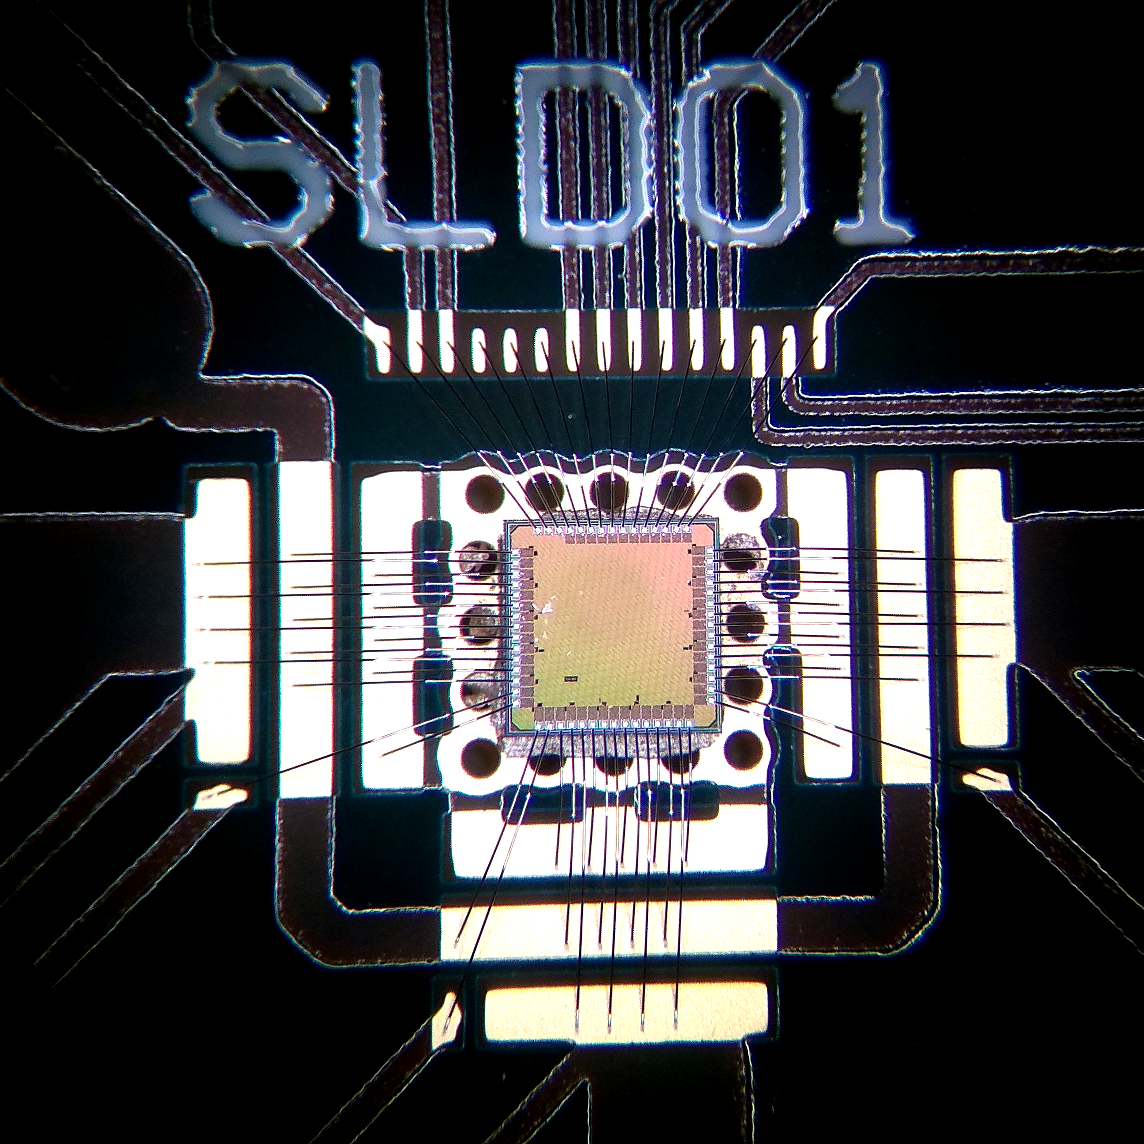
\includegraphics[width=0.32\textwidth]{Immagini/chip05_foto.png}
\hfill
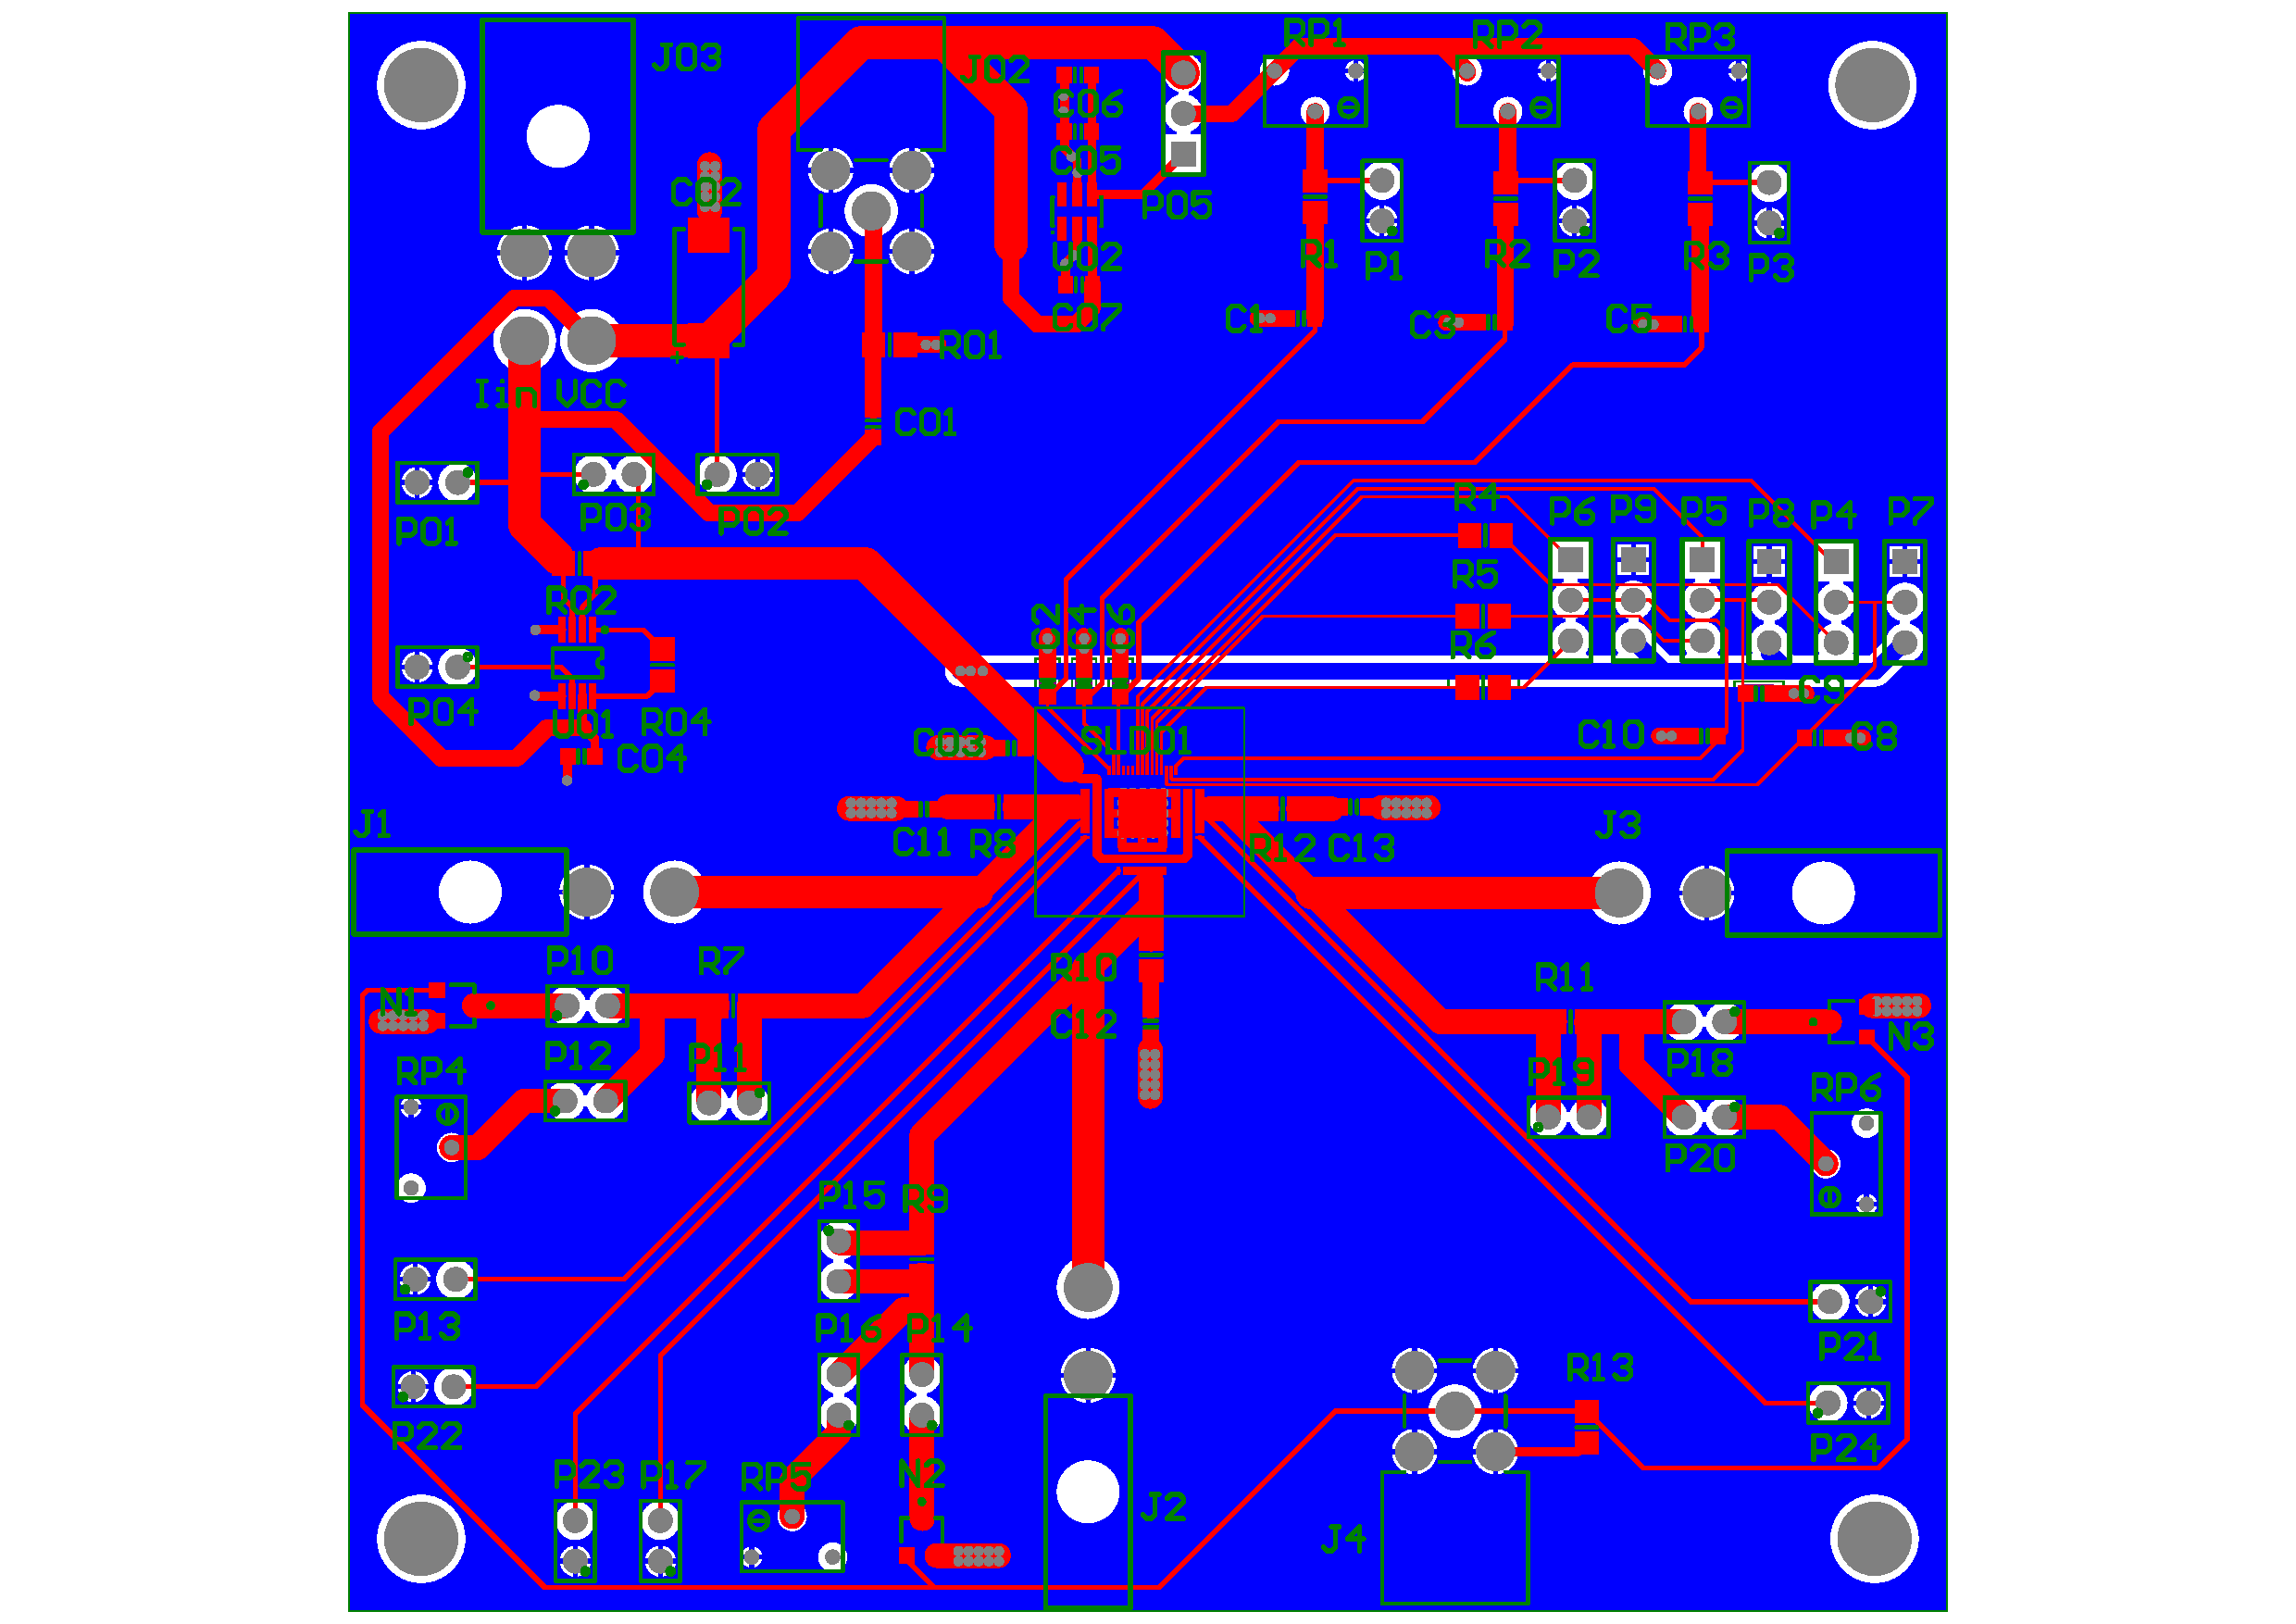
\includegraphics[width=0.32\textwidth]{Immagini/pcb05.pdf}
\caption{La geometria dello ShuntLDO a $0.5\A$ in CMOS a $65\nm$ (sinistra), la foto al microscopio del prototipo montato sulla scheda di test (centro) e il disegno della scheda di test (destra); il chip contiene tre repliche del regolatore e misura circa $2\mm\times 2\mm$ mentre la scheda ha una dimensione di circa $10\cm \times 10\cm$.}
\label{PCB05A}
\end{figure}
Come primo studio abbiamo caratterizzato lo ShuntLDO utilizzando una alimentazione in corrente. Le misure effettuate sono servite ad esaminare l'andamento delle tensioni $\mathrm{V_{in}}$, $\mathrm{V_{out}}$ e $\mathrm{V_{ref}}$ in funzione della corrente in ingresso.

\subsection{Misure in assenza di carico}

\begin{figure}
\centering
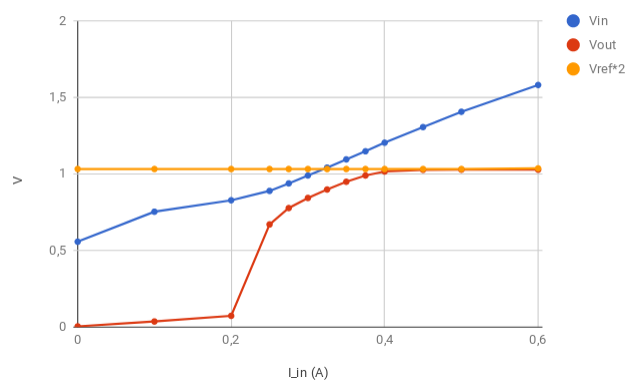
\includegraphics[width=0.75\textwidth]{Immagini/provaSLDO5}
\caption{$\mathrm{V_{in}}$ (blu), $\mathrm{V_{out}}$ (rosso) e $\mathrm{2\times V_{ref}}$ (giallo) in funzione della corrente di ingresso.}
\label{provaSLDO5}
\end{figure}
In Fig.~\ref{provaSLDO5} è riportato il grafico ottenuto variando la corrente in ingresso, in configurazione senza carico al nodo $\mathrm{V_{out}}$ per cui tutta la corrente fornita dall'alimentazione scorre nello shunt scaldandolo significativamente. Questa misura è di particolare interesse per i confronti con la configurazione in cui è presente un carico, sia esso statico o dinamico.
Dato che la parte a sinistra del grafico corrisponde alla situazione in cui il regolatore non è attivo, consideriamo l'andamento asintotico nella zona di regolazione riportando, in particolare, alcuni valori di interesse:
\[
\begin{array}{cccc}
\toprule
%\mathrm{V_{ref}} & \mathrm{V_{out}} & \mathrm{2 \cdot V_{ref}- V_{out}} & \mathrm{R_{eff}} & \mathrm{V_{offset}} \\
%\midrule
%0.516\V & 1.028\V & 8\mV & 2.0\Ohm & 0.40\V \\
\mathrm{V_{ref}} & \mathrm{V_{out}} & \mathrm{R_{eff}} & \mathrm{V_{offset}} \\
\midrule
0.52\V & 1.03\V & 2.0\Ohm & 0.40\V \\
\bottomrule
\end{array}
\]

\subsection{Misure di due ShuntLDO in serie con carico da 4 $\mathrm{\Omega}$}

%La successiva misura di test che è stata eseguita con questo prototipo di shunt, prima del passaggio alla versione da 2A, è un serie di due SLDO entrambi con un carico resistivo di $\mathrm{4 \Omega}$. In questo caso i due elementi hanno $\mathrm{V_{ref}}$ diversi $\mathrm{V_{ref1}=0.497}$ V e $\mathrm{V_{ref2}=0.553 V}$. 
%Ciò non rappresenta un problema in quanto il comportamento "esterno " non ne è influenzato.
Nella configurazione finale, nel ROC per l'esperimento la tensione $\mathrm{V_{ref}}$ viene generata tramite un regolatore di tensione {\em bandgap}\footnote{Una tensione di riferimento `bandgap' \`e ottenuta tramite una circuiteria che fornisce un voltaggio stabile indipendente dalla temperatura e dalle variazioni della tensione di alimentazione in un ampio margine operativo.} alimentato dalla stessa tensione $\mathrm{V_{in}}$ dello ShuntLDO. 
Per scopi diagnostici, tramite la scheda di test, \`e possibile definire la tensione di riferimento $\mathrm{V_{ref}}$ sia tramite un circuito bandgap integrato sulla scheda che si appoggia a $\mathrm{V_{in}}$, sia in maniera indipendente dalle altre alimentazioni dello ShuntLDO fornendo VCC con una sorgente esterna. 
%Sulla scheda di test è presente un bandgap la cui alimentazione può essere separata da quella dello ShuntLDO. Il compito di questo bandgap è quello di generare la tensione di %riferimento $\mathrm{V_{ref}}$, il cui valore può essere regolato con un potenziometro presente sulla scheda di test.
In Fig.~\ref{SLDO5Serie} possiamo vedere il confronto fra il diverso comportamento di due ShuntLDO in serie nel caso in cui VCC, la tensione che alimenta il bandgap, sia fornita esternamente e quello in cui VCC sia cortocircuitata con l'ingresso di $\mathrm{I_{in}}$, trovandosi, dunque, a tensione $\mathrm{V_{in}}$.
In questo confronto va tenuto conto che il bandgap presente sulla scheda di test ha un regime di lavoro compreso tra $2\V$ e $18\V$. 
\begin{figure}
\centering
%\subfloat[][Fondo $WW$.]
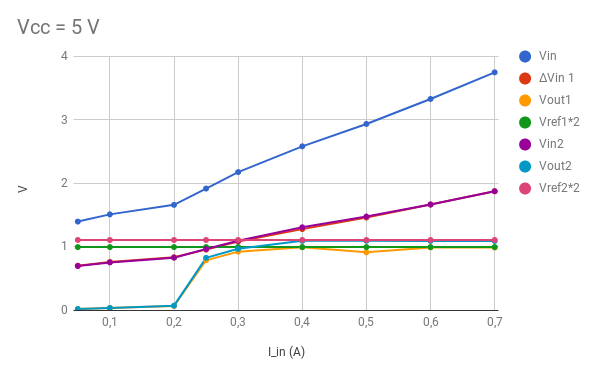
\includegraphics[width=.85\textwidth]{Immagini/SLDO5Serie1}
%\subfloat[][Fondo $WW$.]
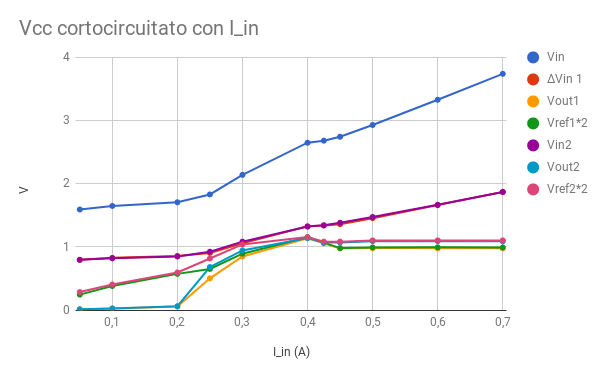
\includegraphics[width=.85\textwidth]{Immagini/SLDO5Serie2}
\caption{Comportamento di due ShuntLDO in serie per due diverse configurazioni di alimentazioni del bandgap integrato sulla scheda che fornisce $\mathrm{V_{ref}}$. In alto i bandgap sono alimentati esternamente, in basso sono alimentati tramite $\mathrm{V_{in}}$.}
\label{SLDO5Serie}
\end{figure}
%Si può notare dai grafici come finto a che la tensione di ingresso non supera circa 1 V il bandgap non riesce a generare il giusto livello di tensione $\mathrm{V_{ref}}$ e ciò ha come conseguenza un $\mathrm{V_{out}}$ non stabile. Si arriva ad una stabilità del $\mathrm{V_{out}}$, solo a tensioni in ingresso più elevate e dunque, con correnti maggiori.
Dai grafici si può notare che, se la tensione di ingresso è inferiore ad $1 \V$, il bandgap non è in grado di generare il giusto livello di tensione $\mathrm{V_{ref}}$, risultando in valori di $\mathrm{V_{out}}$ non stabili. La stabilità di $\mathrm{V_{out}}$ si può ottenere solo con tensioni in ingresso più elevate e, dunque, con correnti maggiori. Questa misura \`e estremamente istruttiva perch\`e illustra l'interazione tra il regolatore e la circuiteria addizionale (in questo caso il bandgap necessario per la tensione di riferimento) nella fase critica dell'accensione. I test di sistema che saranno messi a punto con prototipi pi\`u avanzati dovranno certificare la robustezza dell'approccio utilizzato anche rispetto a queste problematiche.

%magari fare tabellino anche quie
\subsection{Comportamento dinamico}

%\begin{figure}[!hbt]
%\centering
%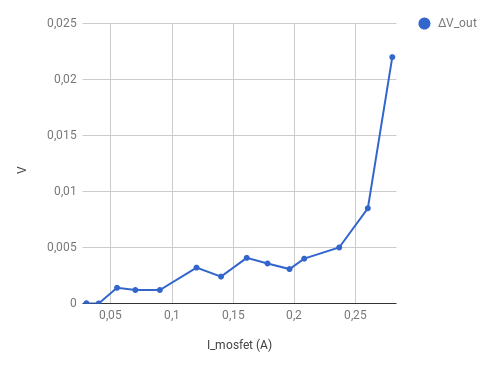
\includegraphics[scale=.5]{Immagini/SLDO5singlepulse}
%\caption{Schema elettrico della circuiteria della scheda di test per lo ShuntLDO a $0.5\A$ dedicata all'emulazione di variazioni rapide del carico grazie ad un mosfet di potenza pilotato da un impulso di gate esterno.}
%\label{SLDO5mosfet}
%\end{figure}
%Prima di passare alla versione da 2A è stata provata una situazione con carico dinamico, per poi riproporla in modo più approfondito ed esaustivo nelle sezioni successive utilizzando però il prototipo da 2A.
Nella scheda di test è presente un mosfet in parallelo all'uscita $\mathrm{V_{out}}$. Il mosfet pu\`o essere pilotato applicando una tensione sul gate. La corrente assorbita dal mosfet si ricava misurando la caduta su una piccola resistenza in serie. Questa circuiteria, il cui schematico \`e visibile in Fig.~\ref{PCB05A}, pu\`o essere utilizzata per emulare variazioni rapide sul carico. 

\begin{figure}[!hbt]
\centering
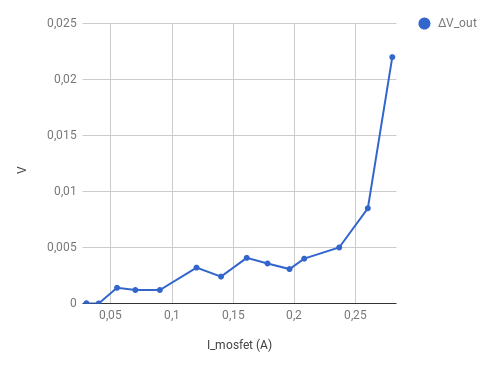
\includegraphics[width=0.75\textwidth]{Immagini/SLDO5singlepulse}
\caption{Entità degli undershoot in tensione in funzione della corrente assorbita dal mosfet.}
\label{SLDO5singlepulse}
\end{figure}
La prima misura di interesse è la sensibilità di $\mathrm{V_{out}}$ alle variazioni veloci di carico.
In Fig.~\ref{SLDO5singlepulse} è riportato l'andamento dell'entit\`a delle fluttuazioni in basso di $\mathrm{V_{out}}$ ({\em undershoot}) in funzione della corrente assorbita dal mosfet.
Le misure sono state effettuate con una alimentazione in corrente $\mathrm{I_{in} = 0.5 A}$, $\mathrm{V_{ref} \sim 0.5 V}$ e carico resistivo su $\mathrm{V_{out}}$ di $4\Ohm$. 
Conoscere il valore della corrente in ingresso è importante poiché, nel momento in cui il carico dinamico e statico assorbono una corrente maggiore di quella totale in ingresso, il sistema smette di funzionare in maniera corretta.

Gli effetti visibili, nelle situazioni in cui $\mathrm{I_{mosfet} + I_{load} > I_{in}}$ dove $\mathrm{I_{load}}$ è la corrente che scorre nel carico resistivo, non sono direttamente legati alle prestazioni dello ShuntLDO. Al contrario si può vedere dal grafico in Fig.~\ref{SLDO5singlepulse} come gli undershoot siano inferiori a $10\mV$ fintantoché $\mathrm{I_{mosfet}}$ rimane al di sotto di $250\mA$, valore oltre il quale $\mathrm{I_{mosfet} + I_{load} > I_{in}}$. In questo caso $\mathrm{I_{load} = \nicefrac{V_{out}}{R} = 250\mA}$. Queste variazioni di  $\mathrm{V_{out}}$ sono perfettamente compatibili con i requisiti.

%Lo stesso tipo di test può essere eseguito mettendo due ShuntLDO in serie e verificando, al variare del carico di uno, che l'altro elemento della catena seriale ne sia influenzato o %meno.
%ed andando a variare dinamicamente il carico di uno dei due, verificando se esternamente queste variazioni siano visibili, e quindi se influenzino l'altro elemento della catena seriale. 
%Dal momento che l'interesse maggiore è per il prototipo a 2 A questo tipo di misura non è stato riportato nel caso dello SLDO da 0.5A, in quanto lo scopo di questa prima parte è quello di introdurre un certo tipo di approccio e  prendere confidenza con gli argomenti trattati.

\section{Lo ShuntLDO da $2\A$}
%\begin{figure}
%\centering
%\includegraphics[scale=.3]{Immagini/PCB2A}
%\caption{.}
%\label{PCB2A}
%\end{figure}
%Rispetto a quanto visto in precedenza, nella versione da 2 A è possibile gestire anche l'offset attraverso un potenziometro, che va ad agire sulla tensione in uscita generata dal bangap, la stessa che viene utilizzata anche per generare $\mathrm{V_{ref}}$ regolando un secondo potenziometro. 

Il prototipo ShuntLDO da $2\A$ \`e, analogamente alla versione precedente, un singolo ASIC realizzato a scopo di verifica e validazione che per\`o, a differenza della versione prototipale a $0.5\A$, contiene una sola replica del regolatore. Per questo chip \`e stata messa a punto una scheda di test analoga a quella di cui alla sezione precedente. In Fig.~\ref{PCB2A} sono visibili la struttura e una foto del chip stesso e il disegno del circuito stampato della scheda di test. 
\begin{figure}
\centering
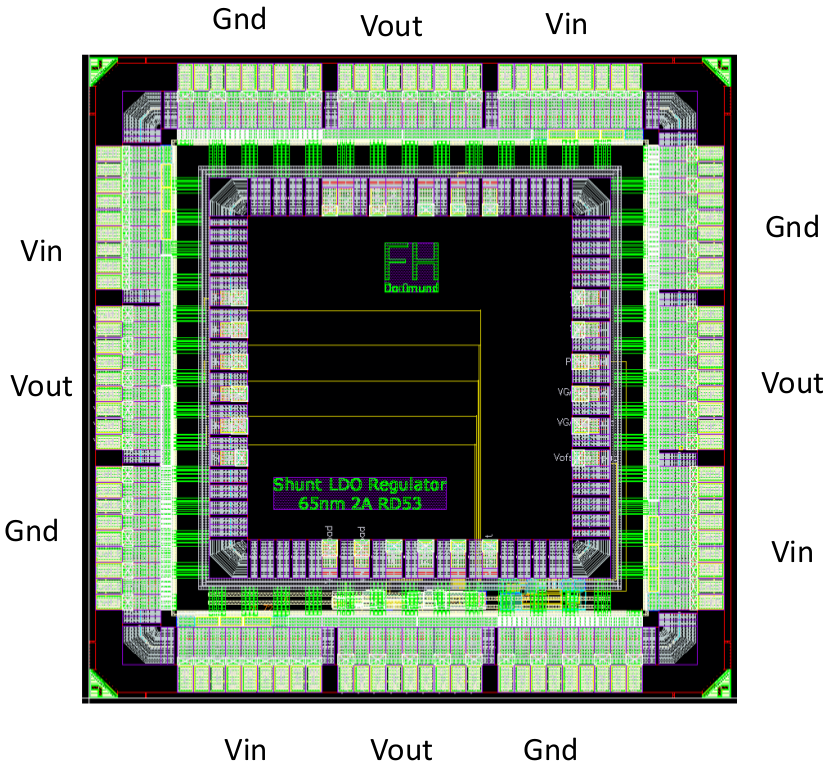
\includegraphics[width=0.32\textwidth]{Immagini/chipSLDO2A.png}
\hfill
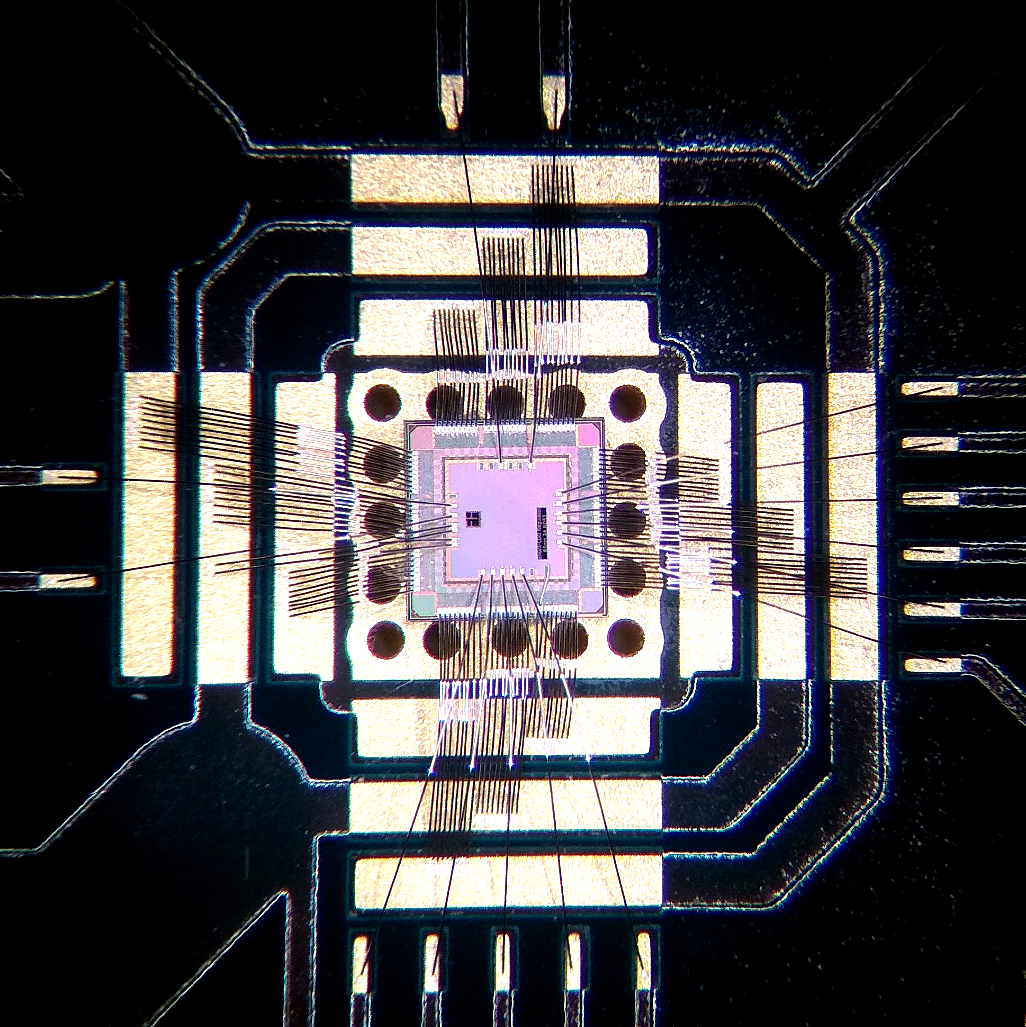
\includegraphics[width=0.32\textwidth]{Immagini/chip2_foto.png}
\hfill
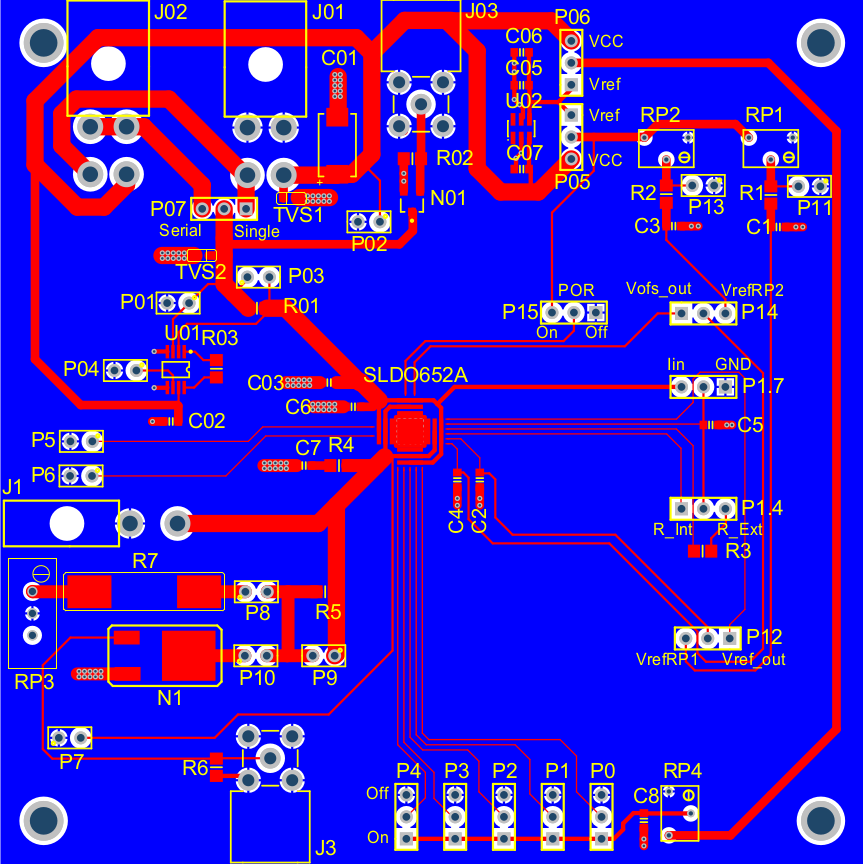
\includegraphics[width=0.32\textwidth]{Immagini/chipcard.png}
\caption{La geometria dello ShuntLDO a $2\A$ in CMOS a $65\nm$ (sinistra), la foto al microscopio del prototipo montato sulla scheda di test (centro) e il disegno della scheda di test (destra); il chip misura $2\mm\times 2\mm$ mentre la scheda ha una dimensione di circa $10\cm \times 10\cm$.}
\label{PCB2A}
\end{figure}
Come abbiamo già detto, un'importante differenza fra la prima versione, con carico massimo da $0.5\A$, e la versione da $2\A$ è la possibilità di modificare $\mathrm{V_{offset}}$ attraverso la scheda di test. $\mathrm{V_{ref}}$ \`e configurabile, tramite bandgap alimentabile anche esternamente, in modo analogo alla scheda di test per il prototipo a $0.5\A$. In questa sezione descriveremo i test effettuati per la caratterizzazione dello ShuntLDO da $2\A$, studiando sia il comportamento con carico statico che dinamico.

\subsection{Comportamento statico}

La caratterizzazione con carico statico è stata ottenuta usando un carico resistivo da $1\Ohm$ su $\mathrm{V_{out}}$, per avere una corrente sul carico pi\`u elevata, con $\mathrm{V_{ref}} = 0.5 \V$ ottenuto tramite il bandgap alimentato esternamente.
I valori misurati di $\mathrm{V_{out}}$, $\mathrm{V_{ref}}$ e $\mathrm{V_{in}}$ al variare della corrente di alimentazione in ingresso sono mostrati in~Fig.~\ref{SLDO2Astatic}.
%La parte di caratterizzazione statica è di nuovo eseguita andando a variare la corrente di alimentazione in ingresso e al contempo misurando $\mathrm{V_{out}}$, $\mathrm{V_{ref}}$ e $\mathrm{V_{in}}$, figura \ref{SLDO2Astatic}.
\begin{figure}
\centering
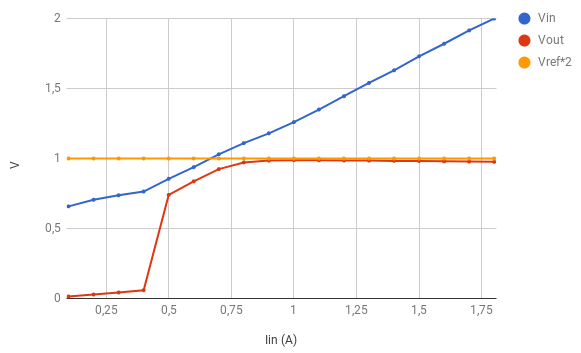
\includegraphics[width=0.9\textwidth]{Immagini/SLDO2Astaticbis}
\caption{Grafico corrente-tensione che riporta gli andamenti di $\mathrm{V_{in}}$, in blu, $\mathrm{V_{ref}\cdot 2}$, in arancione e $\mathrm{V_{out}}$ in rosso.}
\label{SLDO2Astatic}
\end{figure}
Dagli andamenti si può notare che, al momento in cui il circuito si attiva, $\mathrm{V_{out}}$ cerca di raggiungere il valore di $\mathrm{2\times V_{ref}}$, ma nel far questo è limitato da $\mathrm{V_{in}}$, di cui segue l'andamento tra $0.5 \A$ e $0.75 \A$, restando ad una distanza di $\sim 100 \mV$.
Questo comportamento è legato alle caratteristiche del regolatore LDO, il quale al massimo può generare tensioni di uscita tali che $\mathrm{V_{dropout}=V_{in}-V_{out}\sim 0.1-0.2 \V}$.
%Guardando gli andamenti si può notare come, al momento in cui il circuito si attiva, $\mathrm{V_{out}}$ cerca di raggiungere il valore di $1 \V$ (stabilito attraverso $\mathrm{V_{ref}}$), ma nel far questo è limitato da $\mathrm{V_{in}}$ di cui ne segue l'andamento tra $0.5 \A$ e $0.75 \A$ restando ad una distanza di $\sim 100 \mV$. 
%Questo è dovuto alle caratteristiche del regolatore LDO, il quale al massimo può generare tensioni di uscita tali che $\mathrm{V_{dropout}=V_{in}-V_{out}\sim 0.1-0.2 \V}$. 
Considerando gli andamenti asintotici delle tensioni nella zona con $\mathrm{I_{in}}>1\A$ si ottengono i seguenti valori:
%Si può notare che $\mathrm{V_{ref}}$ non è costante nella parte con bassa $\mathrm{I_{in}}$: questo comportamento è dovuto al fatto che, nella fase in cui lo ShuntLDO \`e al di fuori della regione di regolazione, nel ramo di $\mathrm{V_{ref}}$ scorre un po' di corrente che causa una maggiore caduta di tensione del potenziometro e, quindi, una minore tensione all'ingresso di A4 (vd. Fig.~\ref{SLDO2A}).
%Infatti, dato che $\mathrm{V_{ref}}$ si trova all'ingresso del comparatore A1, in una situazione di equilibrio viene confrontata con una tensione molto simile.
%Il comparatore ha una impedenza di ingresso molto grossa e la corrente che scorre in questo sarà, quindi, molto piccola.
%Nella fase di accensione, invece, all'ingresso di A1 si trova una grossa differenza fra + e - e, quindi, una corrente non trascurabile, causa, come visto, della variazione di $\mathrm{V_{ref}}$.

%Questo andamento è stato ottenuto ponendo
%\footnote{Per selezionare il valore voluto è necessario regolare il potenziometro RP1 che si trova in serie al bandgap sulla PBC.} 
%$\mathrm{V_{ref} = 0.5} V$ e applicando un carico resistivo di 1 $\Omega$ a $\mathrm{V_{out}}$. In questa situazione il bandgap è alimentato esternamente con una tensione di 5 V. 
%Come si vede dal grafico \ref{SLDO2Astatic} $\mathrm{V_{ref}}$ non è costante nella parte iniziale, questo può essere dovuto al fatto che nella fase in cui lo shunt LDO non è attivo si ha uno scorrimento di corrente nel ramo di $\mathrm{V_{ref}}$, ciò causa una maggiore caduta di tensione sul potenziometro e quindi una minore tensione all'ingresso di A4. 
%Idealmente, nel ramo di $\mathrm{V_{ref}}$ dovrebbe scorrere una corrente molto piccola in regime di lavoro\footnote{Questo perché nello SLDO il $\mathrm{V_{ref}}$ è in ingresso al comparatore A1 e viene confrontato con una tensione che sarà circa uguale in una situazione di equilibrio. La corrente che scorre tra ingresso + e - sarà piccola, poiché il comparatore in ingresso ha una grossa resistenza.}, mentre al momento dell'accensione, all'ingresso di A1 si ha una notevole differenza tra + e -, e quindi scorrerà una corrente maggiore, questo è causa di una variazione del $\mathrm{V_{ref}}$. Di seguito riportiamo in tabella i valori che si riferiscono al grafico \ref{SLDO2Astatic}: 

\begin{center}
\begin{tabular}{ccccc}
\hline
%$\mathrm{V_{ref}}$ & $\mathrm{V_{out}}$ & $\mathrm{2 \cdot V_{ref}- V_{out}}$ & $\mathrm{R_{eff}}$ & $\mathrm{V_{offset}}$ \\
$\mathrm{V_{ref}}$ & $\mathrm{V_{out}}$ & $\mathrm{R_{eff}}$ & $\mathrm{V_{offset}}$ \\
\hline
%0.500 V & 0.980 V & 20 mV & 0.880 $\Omega$ & 0.40 V\\
0.50 V & 0.98 V & $0.88\Ohm$ & 0.40 V\\
\hline
\end{tabular}
\end{center}
%Infine è interessante notare una leggera flessione del $\mathrm{V_{out}}$ all'aumentare  della corrente in ingresso, questo ha stimolato una riflessione su possibili effetti dovuti a differenze sul riferimento di massa tra regolatore e scheda di test.

Infine è interessante notare una leggera flessione del $\mathrm{V_{out}}$ all'aumentare della corrente in ingresso.
Questa osservazione ha stimolato la ricerca di effetti spuri dovuti all'allestimento di test, come ad esempio la differenze tra il ground del regolatore e quello della scheda di test, che saranno descritti qui di seguito.

\subsection{Effetti spuri dell'allestimento di test}
\label{EffettiSpuri}

\begin{figure}[!ht]
\centering
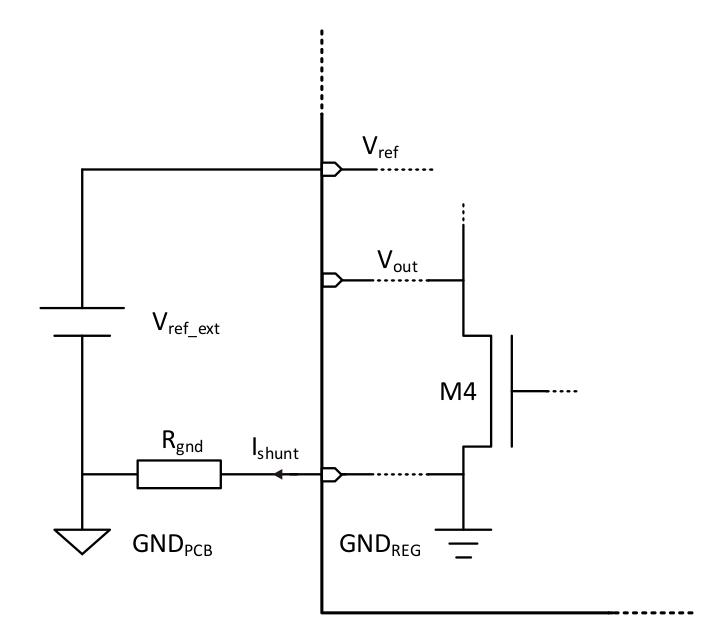
\includegraphics[width=0.75\textwidth]{Immagini/Ground}
\caption{Porzione dello schema elettrico equivalente del prototipo ShuntLDO e della relativa scheda di test in cui \`e resa esplicita la presenza della resistenza spuria denominata $\mathrm{R_{gnd}}$, associata alle microsaldature, tra $\mathrm{GND_{PCB}}$ e $\mathrm{GND_{REG}}$.}
\label{Ground}
\end{figure}
%Prima di procedere oltre è interessante fare alcune riflessioni.% per porre attenzione su un aspetto che influenza le misure. 
A causa delle maggiori correnti in gioco nel prototipo di ShuntLDO da $2\A$ \`e necessario valutare ed, eventualmente, tenere conto degli effetti dovuti a resistenze spurie presenti nella scheda di test. Per la caratterizzazione del prototipo dello ShuntLDO, infatti, si registrano tensioni misurate su terminali appositamente approntati sulla scheda di test. 
Questi terminali sono connessi a loro volta ai terminali del chip tramite microsaldature (vedi Fig.~\ref{PCB2A} centrale) che introducono resistenze in serie, causa di cadute di tensione non trascurabili se attraversate da correnti elevate.
L'entità di queste cadute di tensione dipende dalla resistenza delle microsaldature, dal numero delle stesse\footnote{Le microsaldature si presentano come tante resistenze in parallelo, la resistenza equivalente dipende sia dal valore di resistenza del singolo elemento sia dal numero di elementi in parallelo.} e dalla corrente, e quindi, nel caso di una caratterizzazione con carico statico, si presenta come una differenza di potenziale costante mentre varia con la corrente nel caso di carico dinamico.
\`E utile introdurre una differenziazione tra il nodo di riferimento locale $\mathrm{GND_{PCB}}$ sulla scheda e il nodo di riferimento locale sul regolatore $\mathrm{GND_{REG}}$. Si pu\`o osservare come la frazione della corrente in ingresso scorre attraverso il transistor di shunt (M4), confluisce nella nodo di riferimento del regolatore $\mathrm{GND_{REG}}$ e da qui attraverso le microsaldature nel nodo di riferimento della scheda di test ($\mathrm{GND_{PCB}}$). 
%Questi terminali sono connessi a loro volta ai terminali del chip tramite microsaldature che introducono resistenze in serie le quali causano cadute di tensione non necessariamente trascurabili nel caso in cui le microsaldature siano attraversate da correnti elevate. L'entità di queste cadute di tensione dipende dalla resistenza delle microsaldature, dal numero delle stesse\footnote{Le microsaldature si presentano come tante resistenze in parallelo, la resistenza equivalente dipende sia dal valore di resistenza del singolo elemento sia dal numero di elementi in parallelo.} e dalla corrente, e quindi, nel caso di una caratterizzazione con carico statico, si presenta come una differenza di potenziale costante mentre, nel caso di carico dinamico, varia con la corrente. 
%Per esempio, come visibile nella Fig.~\ref{PCB2A}, \`e utile introdurre una differenziazione tra il nodo di riferimento locale $\mathrm{GND_{PCB}}$ sulla scheda e il nodo di riferimento locale sul regolatore $\mathrm{GND_{REG}}$. Si pu\`o osservare come la frazione della corrente in ingresso scorre attraverso il transistor di shunt (M4), confluisce nella nodo di riferimento del regolatore $\mathrm{GND_{REG}}$ e da qui attraverso le microsaldature nel nodo di riferimento della scheda di test ($\mathrm{GND_{PCB}}$). 
La resistenza di questa linea, rappresentata in Fig.~\ref{Ground} col resistore $\mathrm{R_{gnd}}$, causa una differenza di potenziale tra $\mathrm{GND_{REG}}$ e $\mathrm{GND_{PCB}}$. Di conseguenza la tensione del nodo di regolazione sul chip $\mathrm{V_{out{\_}REG}}$ sar\`a sempre leggermente inferiore a $\mathrm{2\times V_{ref {\_} PCB}}$, dove $\mathrm{V_{ref {\_} PCB}}$ \`e il valore di riferimento fornito esternamente. In particolare, il valore di tensione $\mathrm{V_{out{\_}REG}}$ prodotto dallo ShuntLDO sarà:
\begin{equation}
  \mathrm{V_{out{\_}REG} = 2 \cdot V_{ref{\_}REG} = 2 \cdot ( V_{ref {\_} PCB} - I_{shunt} \cdot R_{gnd} )}.
\end{equation}
Questo effetto è visibile in Fig.~\ref{SLDO2Astatic} dove, all'aumentare della corrente $\mathrm{I_{in}}$, si ha una lieve flessione della tensione in uscita $\mathrm{V_{out{\_}PCB}}$ rispetto a $\mathrm{2 \times V_{ref{\_}PCB}}$ dovuta al fenomeno sopra descritto salvo effetti all'ordine superiore. Facendo un fit lineare di $\mathrm{V_{out{\_}PCB}}$ nella zona di regolazione si ottiene una pendenza equivalente a una resistenza serie di $0.015\Ohm$ risultante non esclusivamente dalle microsaldature, ma anche al contributo aggiuntivo dovuto alla resistenza delle piste e dei connettori.
%Questo effetto è visibile in~Fig.~\ref{SLDO2Astatic} dove, all'aumentare della corrente $\mathrm{I_{in}}$, si ha una lieve flessione della tensione in uscita $\mathrm{V_{out{\_}PCB}}$ rispetto a $2 \times V_{ref{\_}PCB}$ dovuta al fenomeno sopra descritto salvo effetti all'ordine superiore. Facendo un fit lineare di $\mathrm{V_{out{\_}PCB}}$ nella zona di regolazione si ottiene una pendenza equivalente a una resistenza serie di $0.015\Ohm$ risultante non esclusivamente dalle microsaldature, ma anche al contributo aggiuntivo dovuto alla resistenza delle piste e dei connettori.

%%microsaldature in serie a 1 Ohm trascurabili

%----da qui tagliare?
%Per misure pi\`u accurate la scheda di test prevede anche appositi terminali di monitoraggio $\mathrm{V_{out{\_}Sense}}$ e $\mathrm{I_{out {\_} Sense}}$,
%%indicati sulla scheda di test con P5 e P6, rispettivamente.
%collegati, rispettivamente, a $\mathrm{V_{out{\_}REG}}$ e a $\mathrm{GND_{REG}}$ sul regolatore. Essendo rami in cui non scorre corrente, l'effetto resistivo delle connessioni è eliminato ed è possibile misurare il valore di tensione del GND locale.
%
%\begin{figure}
%\centering
%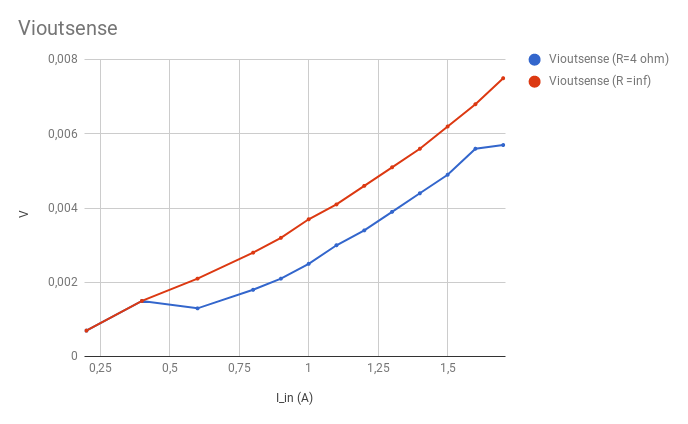
\includegraphics[scale=.4]{Immagini/Viout}
%\caption{Andamento della tensione di $\mathrm{GND_{REG}}$, riferimento locale del chip, rispetto al $\mathrm{GND_{PCB}}$, riferimento locale della  scheda di test, al variare della corrente di alimentazione del circuito per due valori del carico statico connesso a $\mathrm{V_{out{\_}PCB}}$:  $4\Omega$ (curva rossa) e assenza di carico (curva blu). Si precisa che solo per $\mathrm{I_{in}}$ al di sopra di $\sim 750\mA$ il circuito \`e in zona di regolazione.}
%\label{VioutSense}
%\end{figure}
%Si è proceduto quindi a misurare il valore di tensione sul pin $\mathrm{I_{out{\_}Sense}}$ al variare della corrente di alimentazione $\mathrm{I_{in}}$. 
%La misura è stata eseguita per due diversi valori di carico statico connesso al nodo $\mathrm{V_{out{\_}PCB}}$, $4\Omega$ e in assenza di carico, per cui il circuito fra $\mathrm{V_{out{\_}PCB}}$ e $\mathrm{GND_{PCB}}$ è aperto, presentandosi come una resistenza molto grande.
%%$4 \Omega$ e $\infty$, con il valore infinito si intende la configurazione in cui il carico è assente e dunque il circuito tra $\mathrm{V_{out}}$ e GND è aperto, presentandosi di fatto come una resistenza infinita. 
%Gli andamenti di $\mathrm{I_{out {\_} Sense}}$ in funzione di $\mathrm{I_{in}}$ per le due configurazioni sono riportati in Fig.~\ref{VioutSense}.
%La pendenza delle due curve riportate è la stessa, pari a $\sim 4\mOhm$, e ci fornisce un'indicazione del valore resistivo $\mathrm{R_{gnd}}$ delle microsaldature, mentre la separazione tra le due curve risulta alla diversa corrente che lo shunt riversa nel nodo $\mathrm{GND_{REG}}$. Maggiore è la corrente richiesta dal carico, minore è la corrente che attraversa lo shunt e quindi il valore della differenza tra $\mathrm{GND_{REG}}$ e $\mathrm{GND_{PCB}}$.
%La separazione tra le curve, pari a $1\mV$ circa, corrisponde alla caduta di tensione causata dalla diversa corrente che scorre nello shunt nei due casi:
%\begin{equation}
%\mathrm{\Delta V = \Delta I_{shunt} \cdot R_{gnd} = 0.250\A \cdot 4\mOhm = 1\mV}.
%\end{equation}
%All'attento osservatore non sfuggir\`a che le due curve di Fig.~\ref{VioutSense} non sono perfettamente rettilinee. Dato che la misura in oggetto \`e una stima diretta di $\mathrm{I_{shunt}\times R_{gnd}}$ e che l'andamento parabolico \`e presente anche in assenza di carico, situazione in cui $\mathrm{I_{shunt}=I_{in}}$, l'ipotesi \`e che il valore di $\mathrm{R_{gnd}}$ sia indirettamente dipendente da $\mathrm{I_{in}}$ per effetti di temperatura dato che lo ShuntLDO scalda in modo consistente. Queste misure saranno ripetute in condizioni di temperatura controllata per verificare l'ipotesi.
%In figura \ref{VioutSense} è possibile vedere come le due diverse configurazioni di carico influenzino la misura con un offset. 
%Infatti nei due casi la pendenza è la stessa e dà un'indicazione del valore resistivo R dei wire bond, l'offset invece rispecchia il fatto che lo spostamento di tensione è dato dalla corrente che scorre verso il GND del chip, che nel caso in cui il carico richieda più corrente diminuisce.
%Ad esempio ad 1 A con il carico resistivo da 4 $\Omega$, la corrente che effettivamente scorre verso GND nello shunt è 0.75 A (questo nel caso $\mathrm{V_{out} = 1 V}$).

%\par \begin{center} !!! CHE ROBA E'?! CAPTION O ALMENO DESCRIZIONE NEL TESTO !!! \end{center} \par
%
%\begin{center}
%\begin{tabular}{cccc}
%\hline
%$\mathrm{R_{rossa}}$  & $\mathrm{R_{blu}}$ & $\mathrm{Offset_{rosso}}$ & $\mathrm{Offset_{blu}}$\\
%\hline
%4 m$\Omega$ & 4 m$\Omega$ & -1 mV & -2 mV\\
%\hline
%\end{tabular}
%\end{center}

Il valore della resistenza equivalente è molto piccolo e, come detto, dipende in prima approssimazione dal numero di microsaldature.
Fintantoché lo ShuntLDO è utilizzato come circuito a se stante su una scheda di test, dato che non ci sono problemi di spazio, è possibile utilizzare un gran numero di connessioni per ridurre al minimo differenze tra $\mathrm{GND_{PCB}}$ e $\mathrm{GND_{REG}}$, in modo da rendere trascurabile il fenomeno. 
Pi\`u in generale, questa istruttiva misura suggerisce che grande cura dovr\`a essere posta nel disegno finale dei moduli dell'IT e in particolare nella ridondanza delle connessioni dal momento che si tratter\`a di dispositivi a corrente relativamente alta in cui gli eventuali effetti spuri vanno attentamente valutati e, se possibile, minimizzati se non completamente eliminati.

\subsection{La regolazione di  $\mathrm{V_{offset}}$}
\label{Voffset}

Torniamo adesso a considerare la possibilità, nella versione da 2 A, di regolare esternamente il $\mathrm{V_{offset}}$. 
Dal momento che $\mathrm{V_{in}}$ dello ShuntLDO deve trovarsi, per funzionare al meglio, $200-300\mV$ al di sopra di $\mathrm{V_{out}=2\times V_{ref}}$, una tensione di offset alta consente di raggiungere la zona di regolazione prima, a parit\`a di $\mathrm{I_{in}}$, contenendo cos\`i i consumi totali, sempre che la corrente circolante sia sufficiente per le esigenze del carico da alimentare.
%Dal momento che $\mathrm{V_{in}}$ dello ShuntLDO deve trovarsi, per funzionare al meglio, $200-300\mV$ al di sopra di $\mathrm{V_{out}=2\times V_{ref}}$, una tensione di offset alta consente di raggiungere la zona di regolazione prima a parit\`a di $\mathrm{I_{in}}$ contenendo cos\`i i consumi totali sempre che la corrente circolante sia sufficiente per le esigenze del carico da alimentare.
Si può verificare questo fenomeno misurando la tensione di uscita del regolatore $\mathrm{V_{out}}$, per diversi valori di $\mathrm{V_{offset}}$, al variare di $\mathrm{I_{in}}$, come mostrato in Fig.~\ref{VoutVsVoffset}.
\begin{figure}
\centering
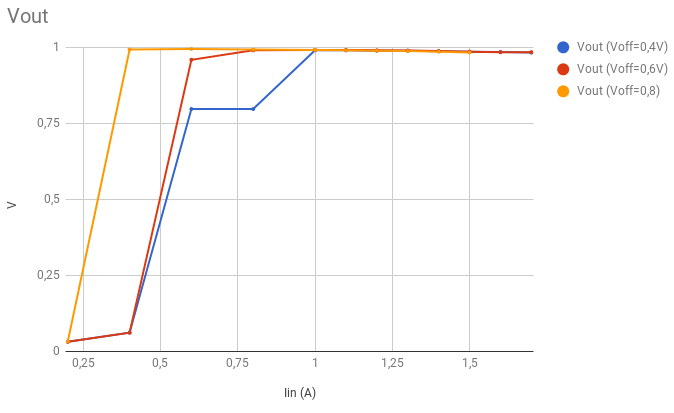
\includegraphics[width=0.9\textwidth]{Immagini/VoutVsVoffset}
\caption{Andamento di $\mathrm{V_{out}}$ al variare della corrente in ingresso per differenti valori di $\mathrm{V_{offset}}$.}
\label{VoutVsVoffset}
\end{figure}

Dalla misura di $\mathrm{V_{in}}$ al variare della corrente in ingresso, mostrata in Fig.~\ref{VinVsVoffset}, è possibile ricavare, con un fit lineare nella regione di regolazione del circuito, l'intercetta con l'asse verticale, corrispondente all'offset effettivo dello ShuntLDO. 
%Dalla misura di $\mathrm{V_{in}}$ al variare della corrente in ingresso mostrata in Fig.~\ref{VinVsVoffset} è possibile ricavare, con un fit lineare nella regione di regolazione del circuito, l'intercetta con l'asse verticale, corrispondente all'offset effettivo dello ShuntLDO. 
\begin{figure}
\centering
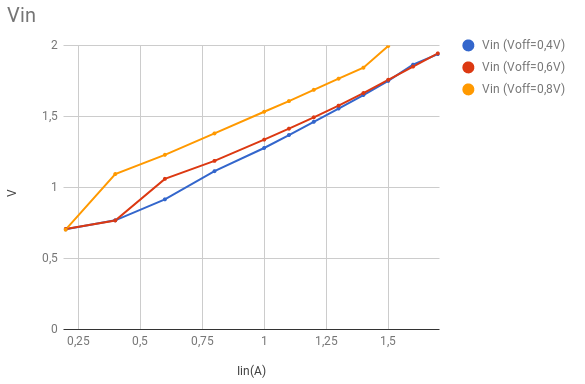
\includegraphics[width=0.9\textwidth]{Immagini/VinVsVoffset}
\caption{Andamento di $\mathrm{V_{in}}$ al variare della corrente in ingresso per differenti valori di $\mathrm{V_{offset}}$.}
\label{VinVsVoffset}
\end{figure}

%Questi valori sono riportati nella tabella seguente:
I valori ottenuti dal fit delle misure sono:

\begin{center}
\begin{tabular}{rccc}
\hline
Offset nominale & $0.4\V$ & $0.6\V$ & $0.8\V$\\
\hline
Offset effettivo & $0.35\V$ & $0.54\V$ & $0.76\V$\\
\hline
\end{tabular}
\end{center}
%\[
%\begin{array}{ccc}
%
%\toprule
%\mathrm{Offset 0.4 V} & \mathrm{Offset 0.6 V} & \mathrm{Offset 0.8 V} \\
%
%\midrule
%
%0.352 V & 0.539 V & 0.756 V \\
%
%\bottomrule
%\end{array}
%\]

%Come si può vedere il valore effettivo è sempre leggermente minore di quello impostato. Questo fenomeno è stato osservato anche nelle misure eseguite sullo ShuntLDO presente all'interno del ROC RD53A e che descriveremo più avanti e non sono ancora chiare le cause. Altra anomalia osservabile nel grafico \`e la differente pendenza delle varie curve che, per\`o, dovrebbe rimanere invariata. I dati mostrano altres\`i una correlazione tra pendenza e offset le cui cause sono anch'esse ignote al momento. %magari mettere referenza a Fig.~\ref{OffsetKaragounis}
Come si può vedere il valore effettivo è sempre leggermente minore di quello impostato. Questo fenomeno è stato osservato anche nelle misure eseguite sullo ShuntLDO presente all'interno del ROC RD53A e che descriveremo più avanti, ma non ne sono ancora chiare le cause. Altra anomalia osservabile nel grafico \`e la differente pendenza delle varie curve che dovrebbe rimanere invariata dato che il valore di $\mathrm{R_{eff}}$ è lo stesso per tutte le misure. I dati mostrano altres\`i una correlazione tra pendenza e offset le cui cause sono anch'esse ignote al momento. %magari mettere referenza a Fig.~\ref{OffsetKaragounis}
%\FloatBarrier

%
% -------------------------------------------------------------------------------------------------------
%
